% for the et figures, pbias on top (hargreaves, pen, priestly), and nash sut on bottom (ditto)

\begin{landscape}
	\begin{tabular}{c c c l} % left bottom right top
		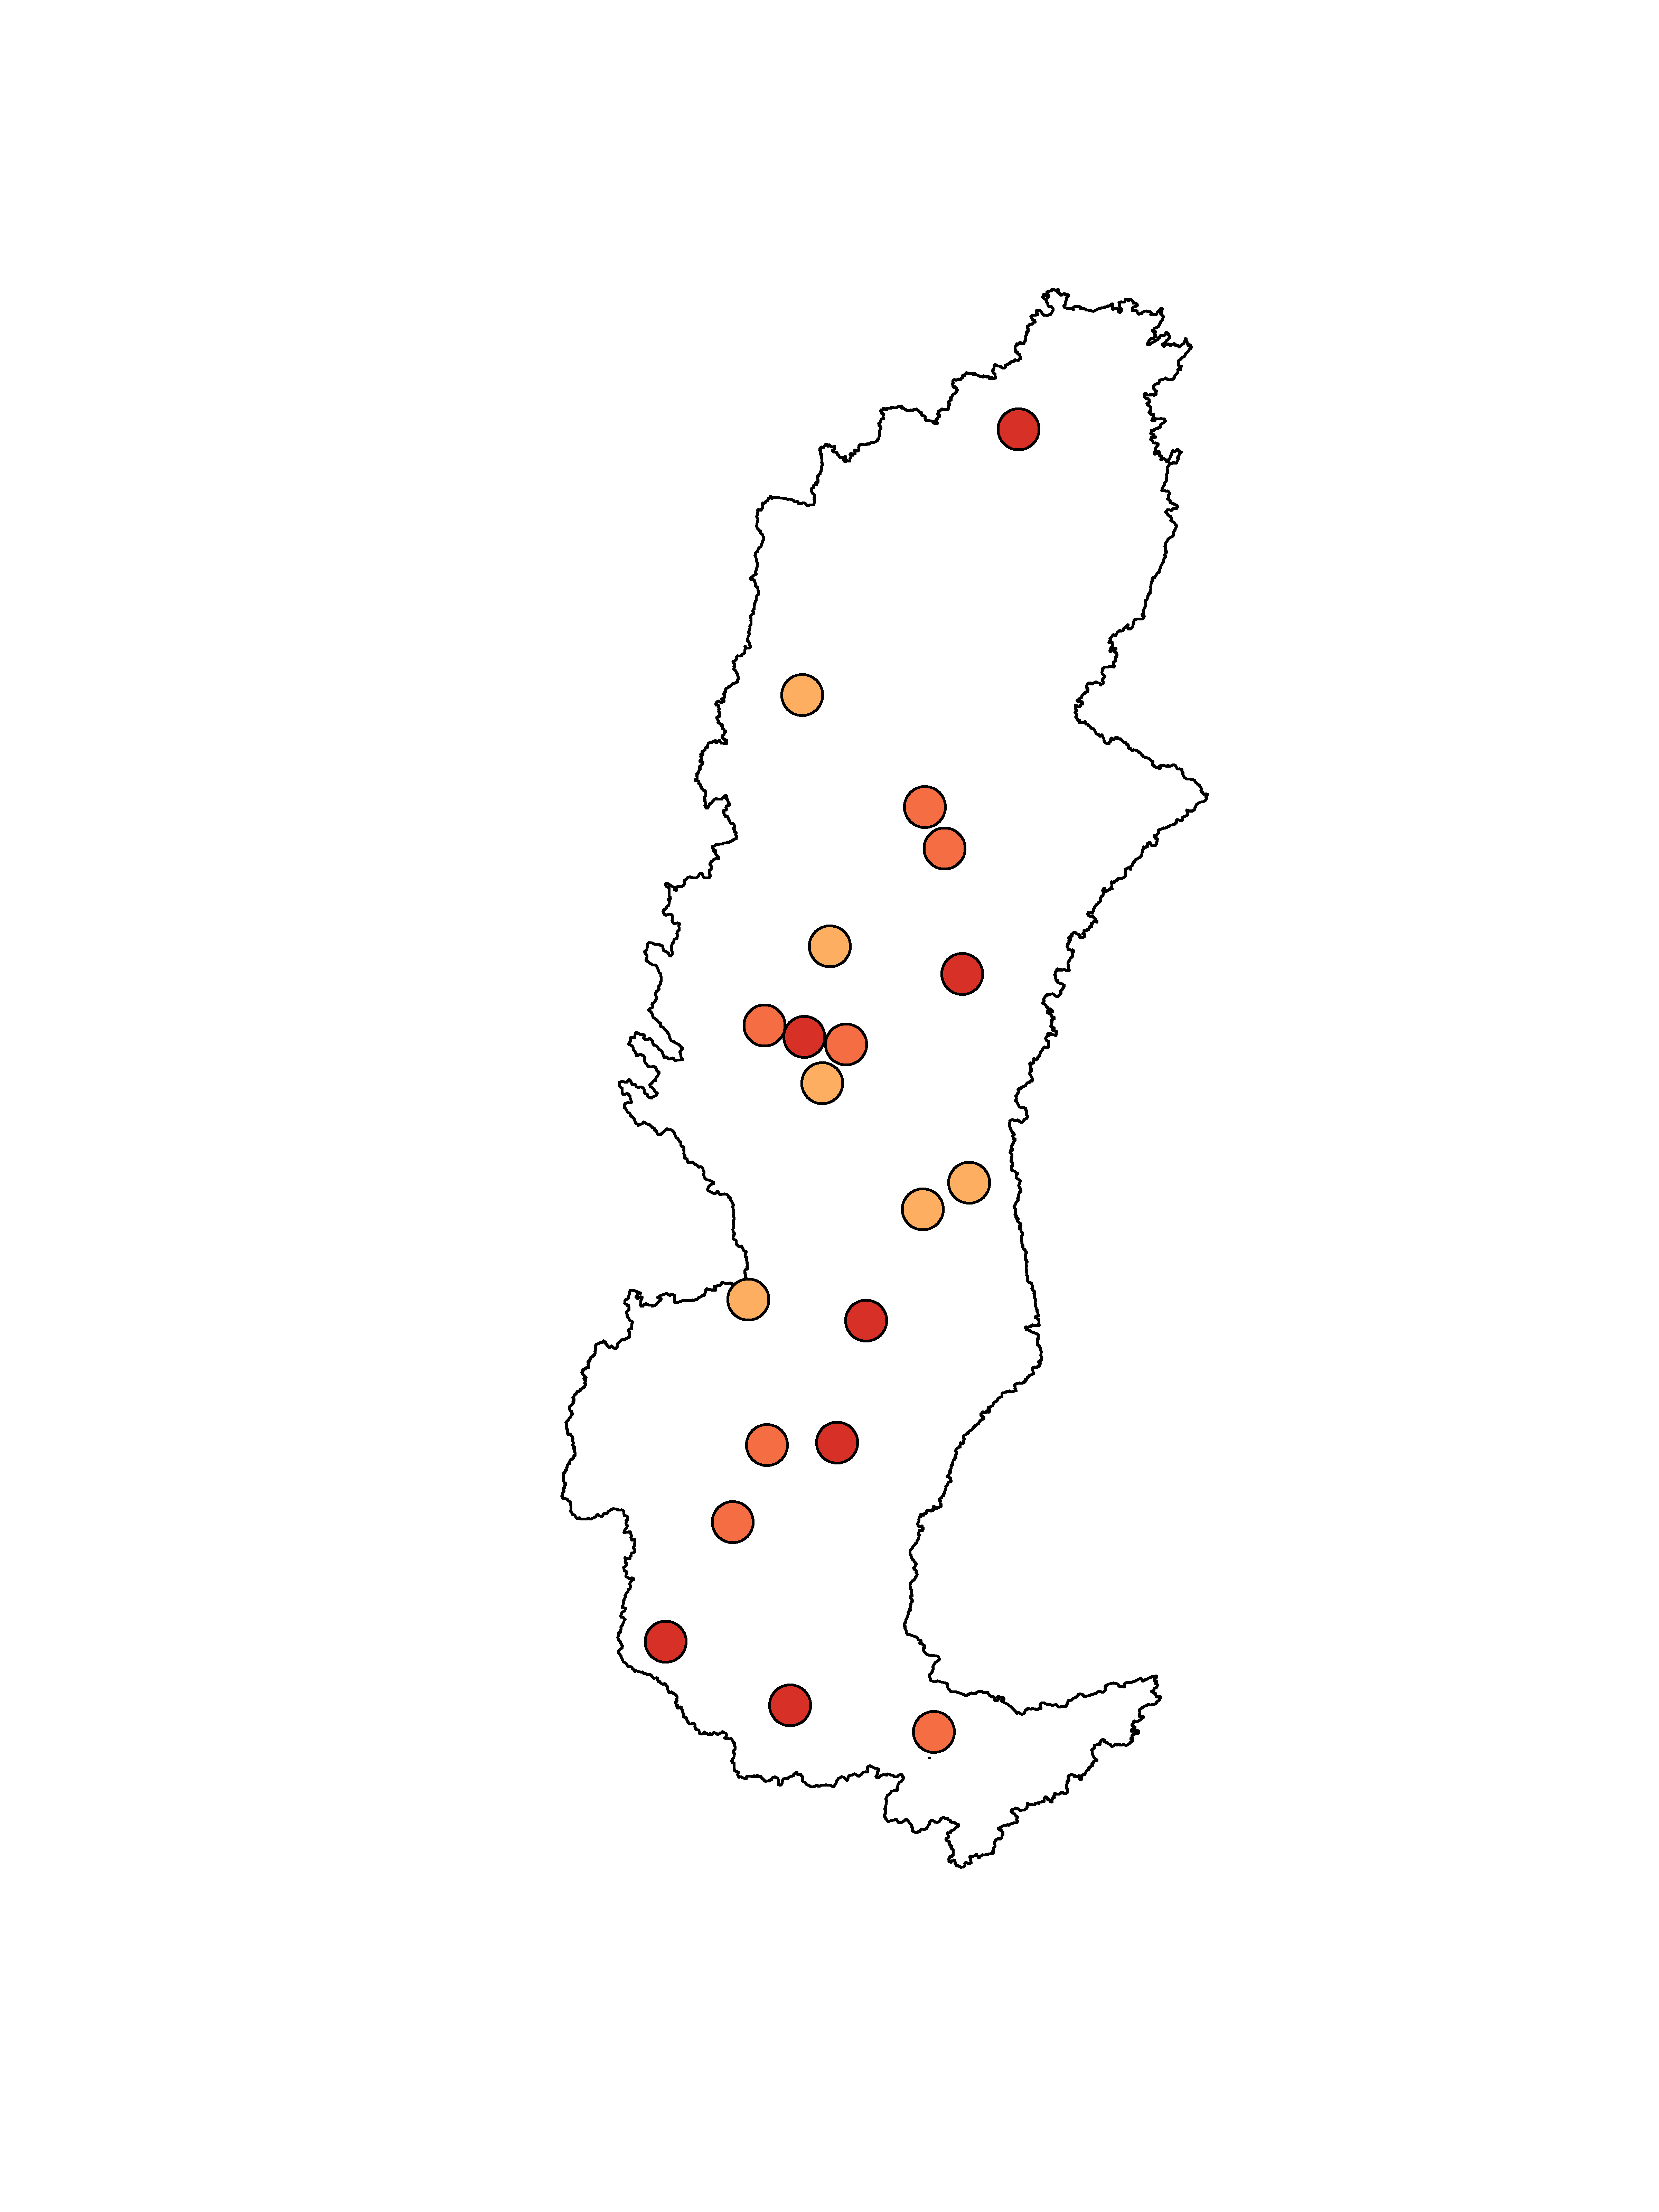
\includegraphics[trim= 4cm 2cm 1cm 2cm, clip, scale = 0.35]{./img/pbias_harg} &
			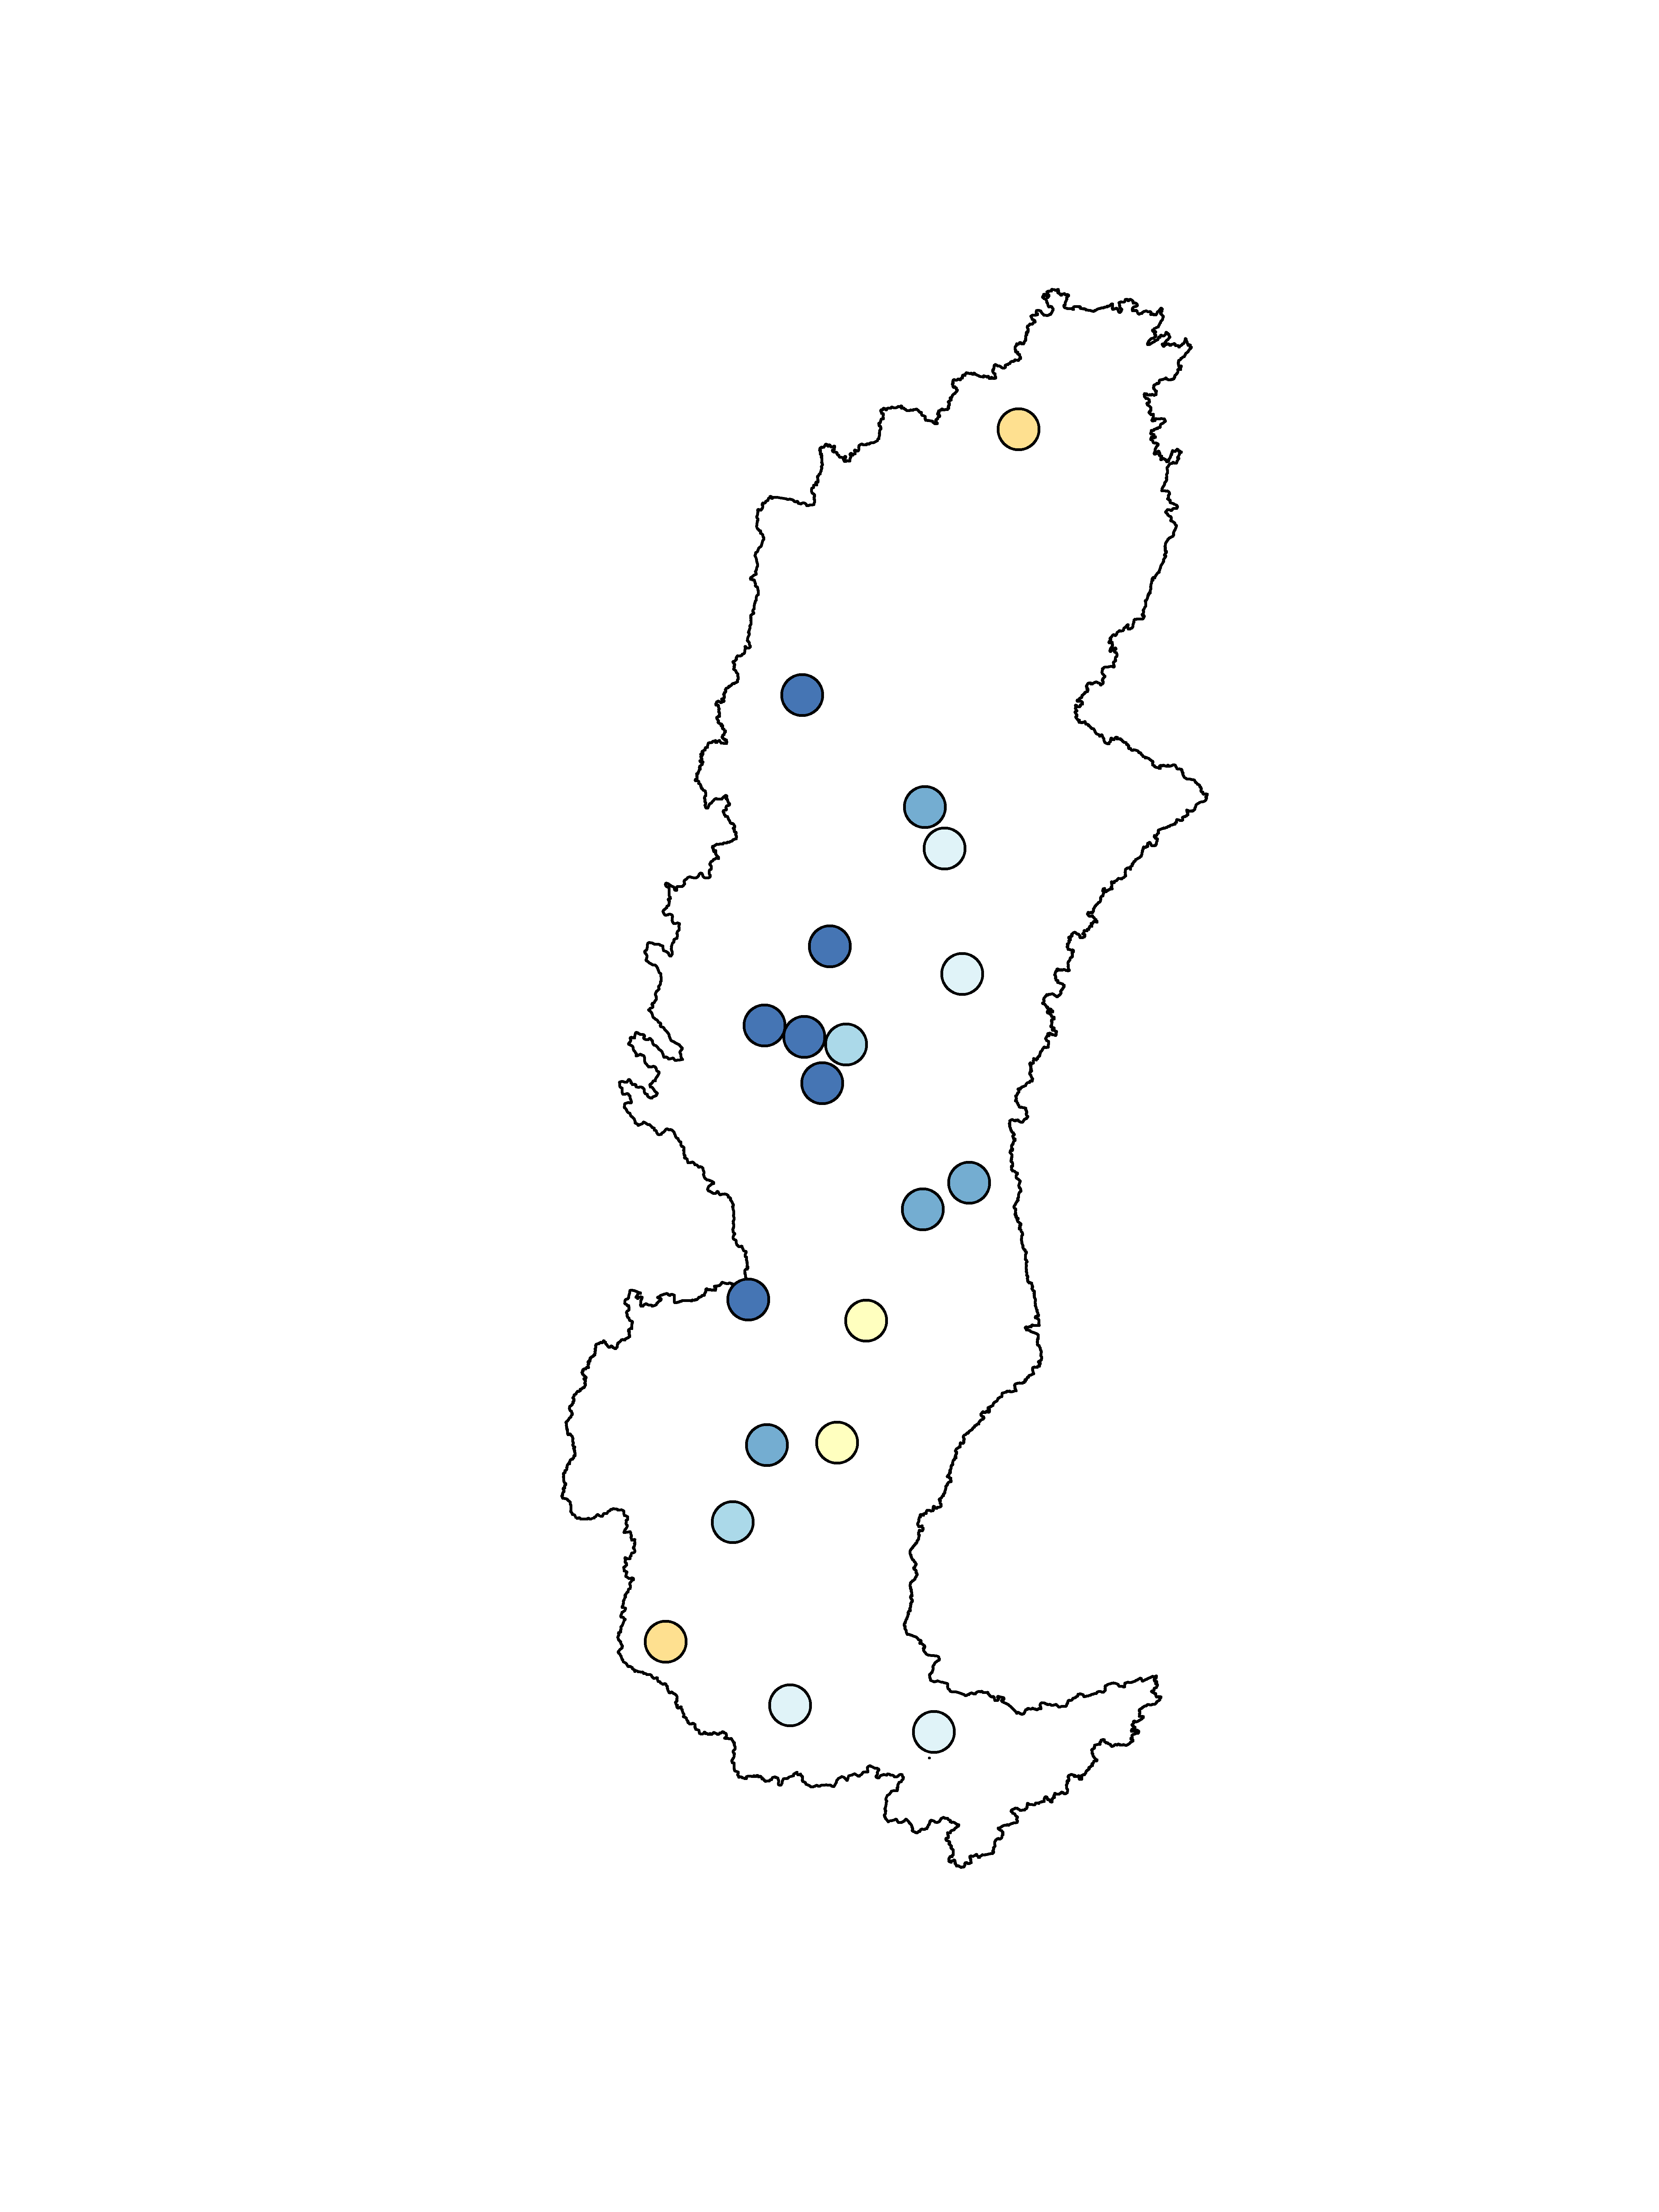
\includegraphics[trim= 4cm 2cm 1cm 2cm, clip, scale = 0.35]{./img/pbias_penman} &
				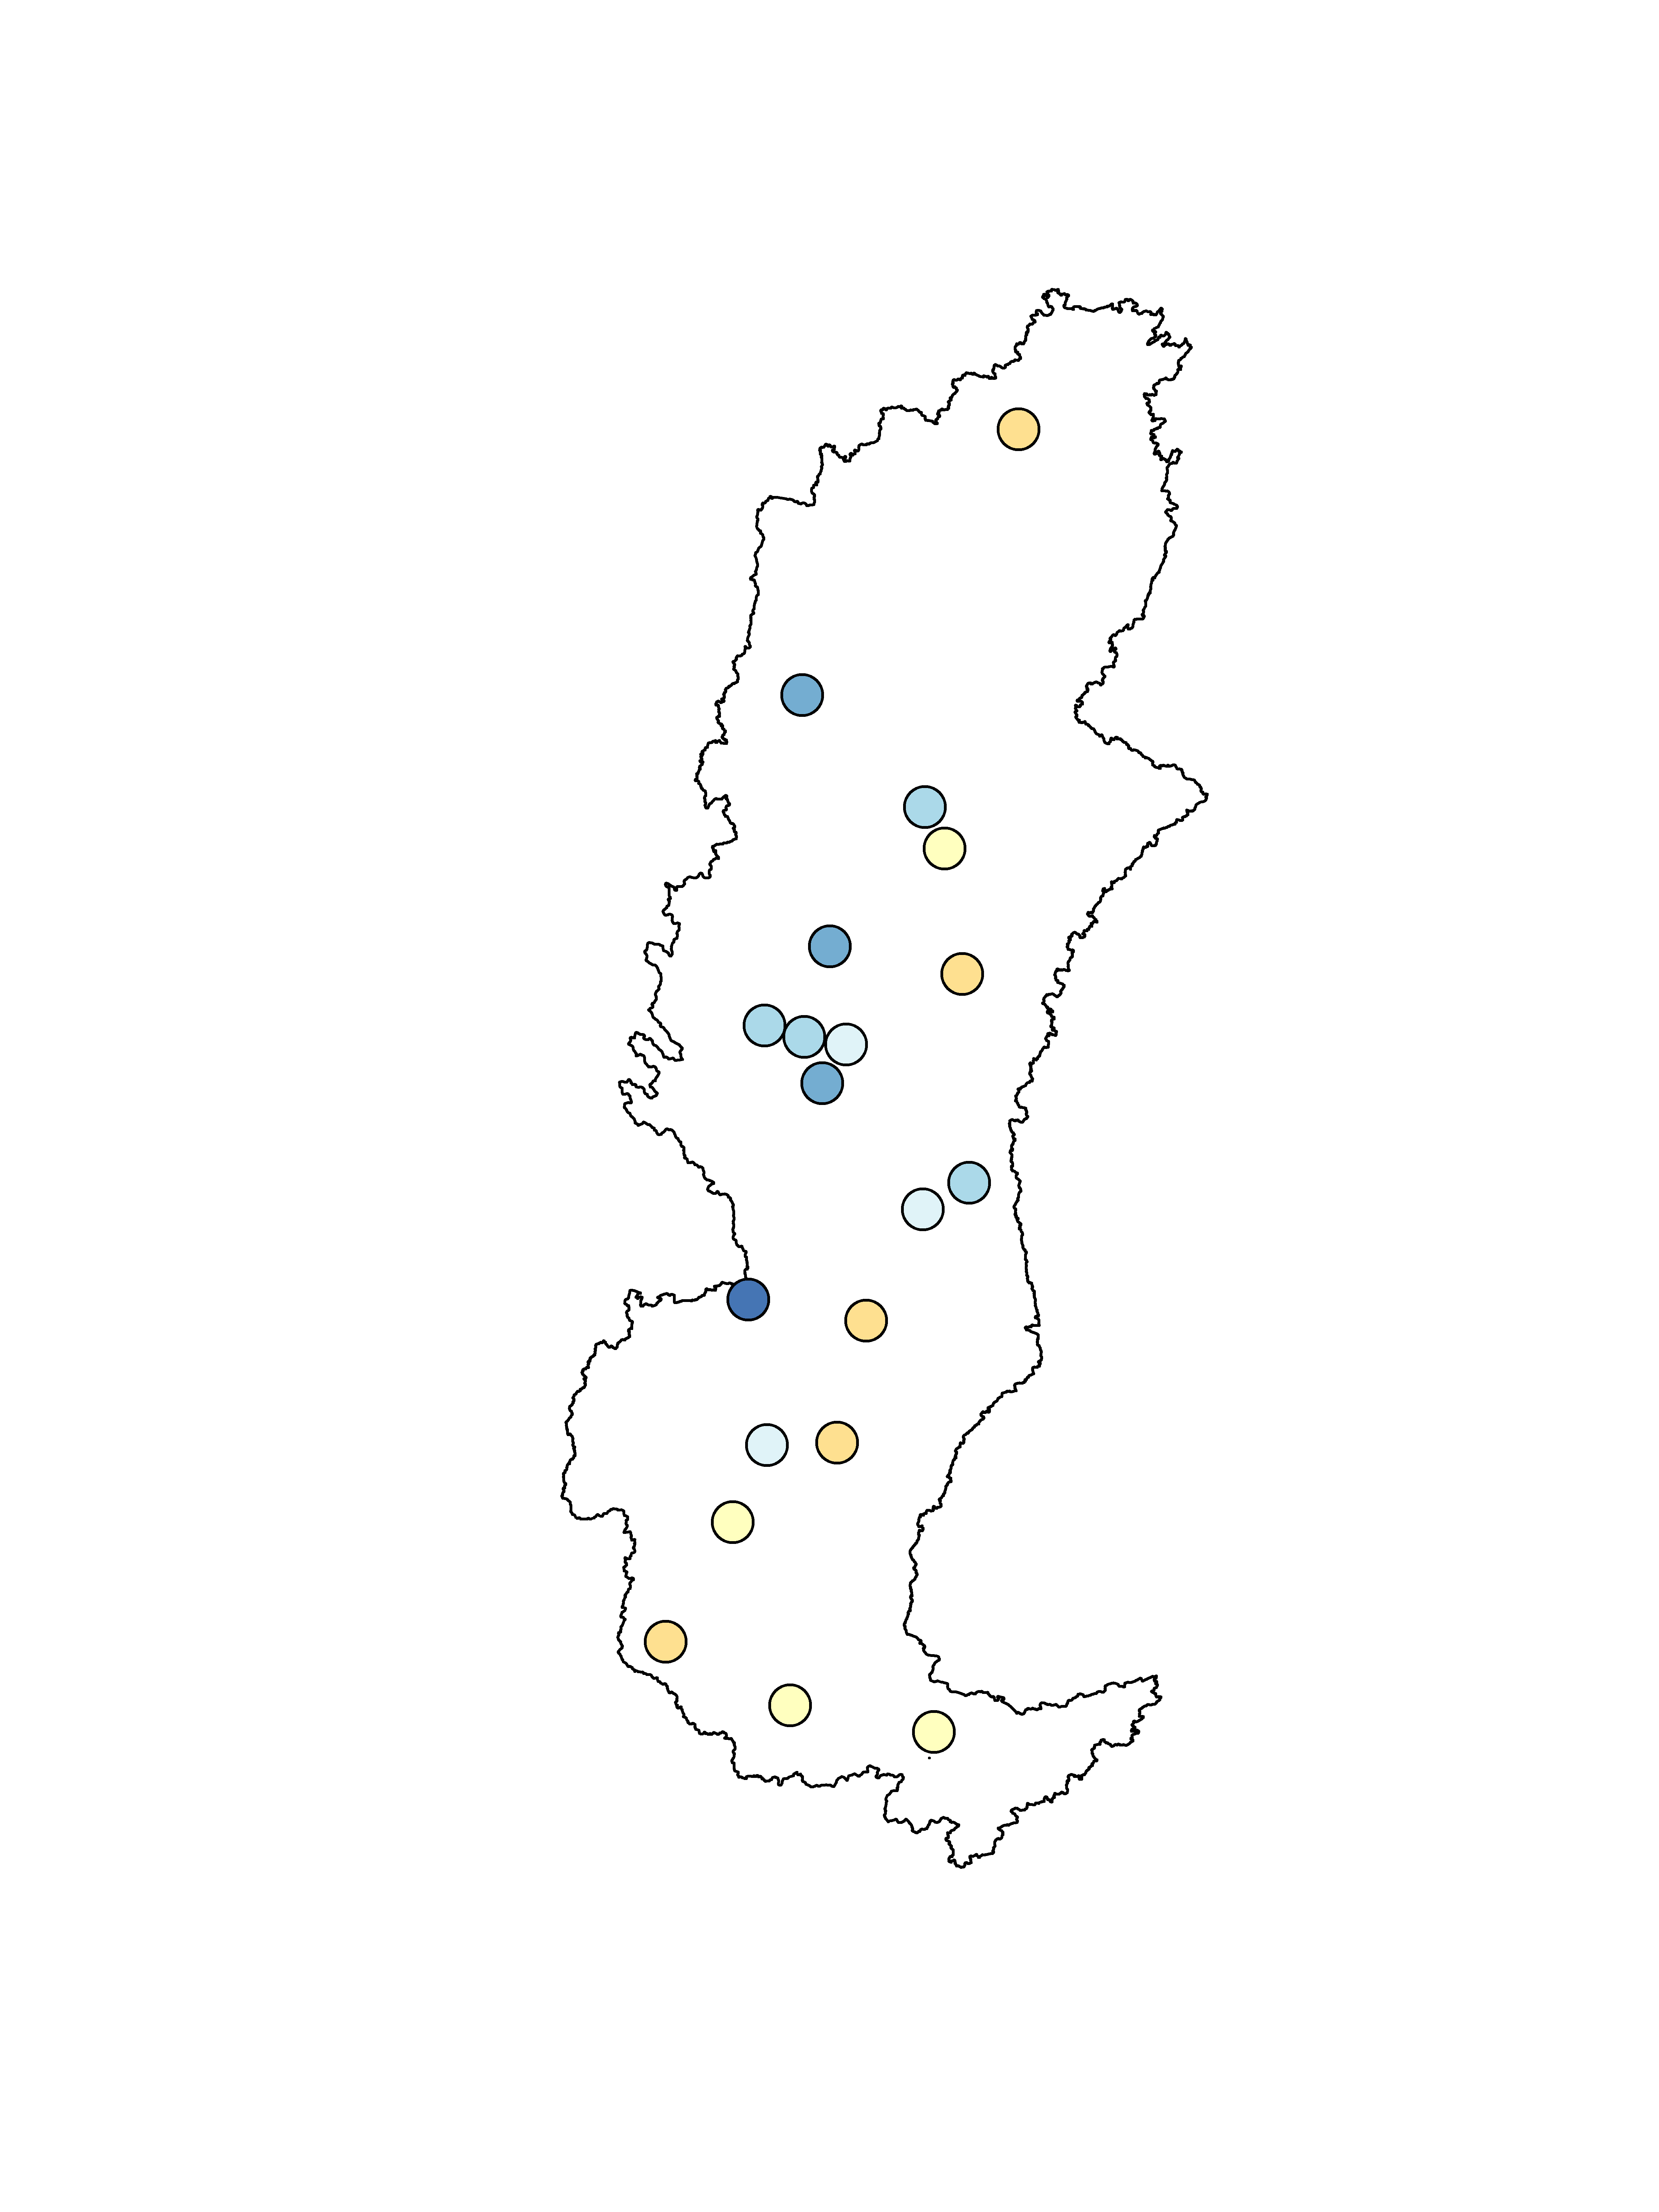
\includegraphics[trim= 4cm 2cm 1cm 2cm, clip, scale = 0.35]{./img/pbias_priestley} &
					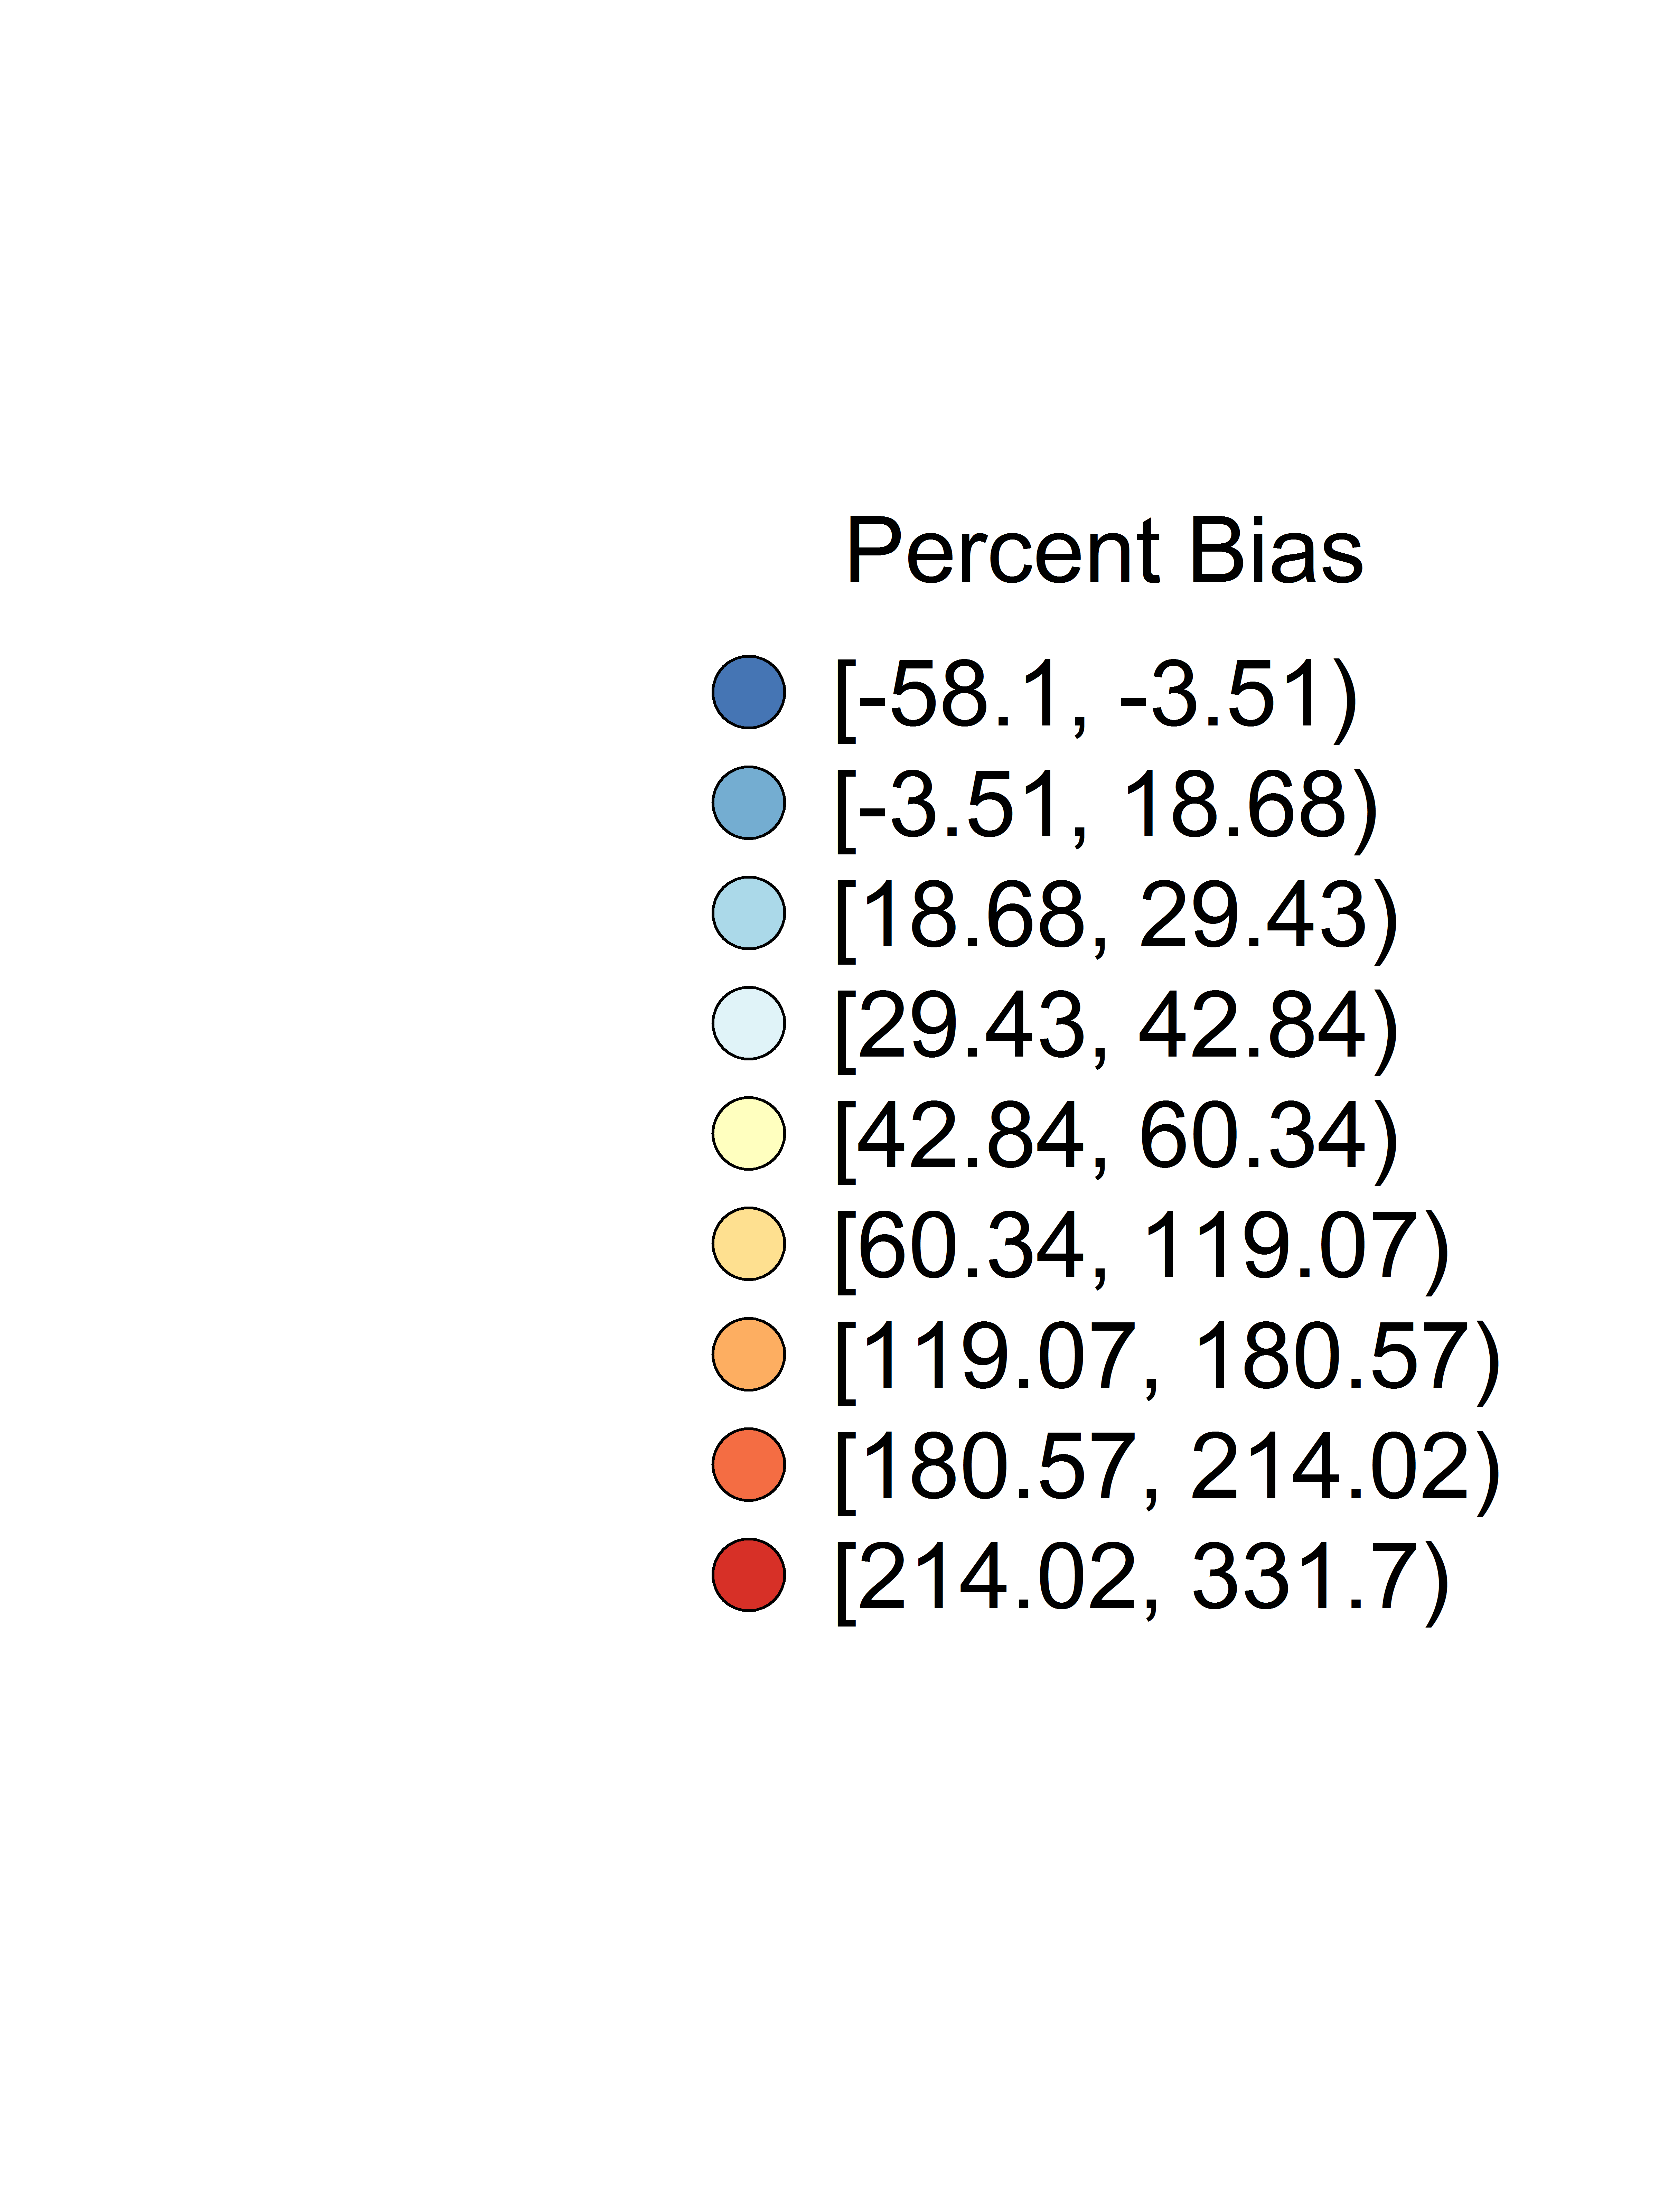
\includegraphics[trim= 5cm 2cm 0cm 3cm, clip, scale = 0.3]{./img/pbias_legend} \\
		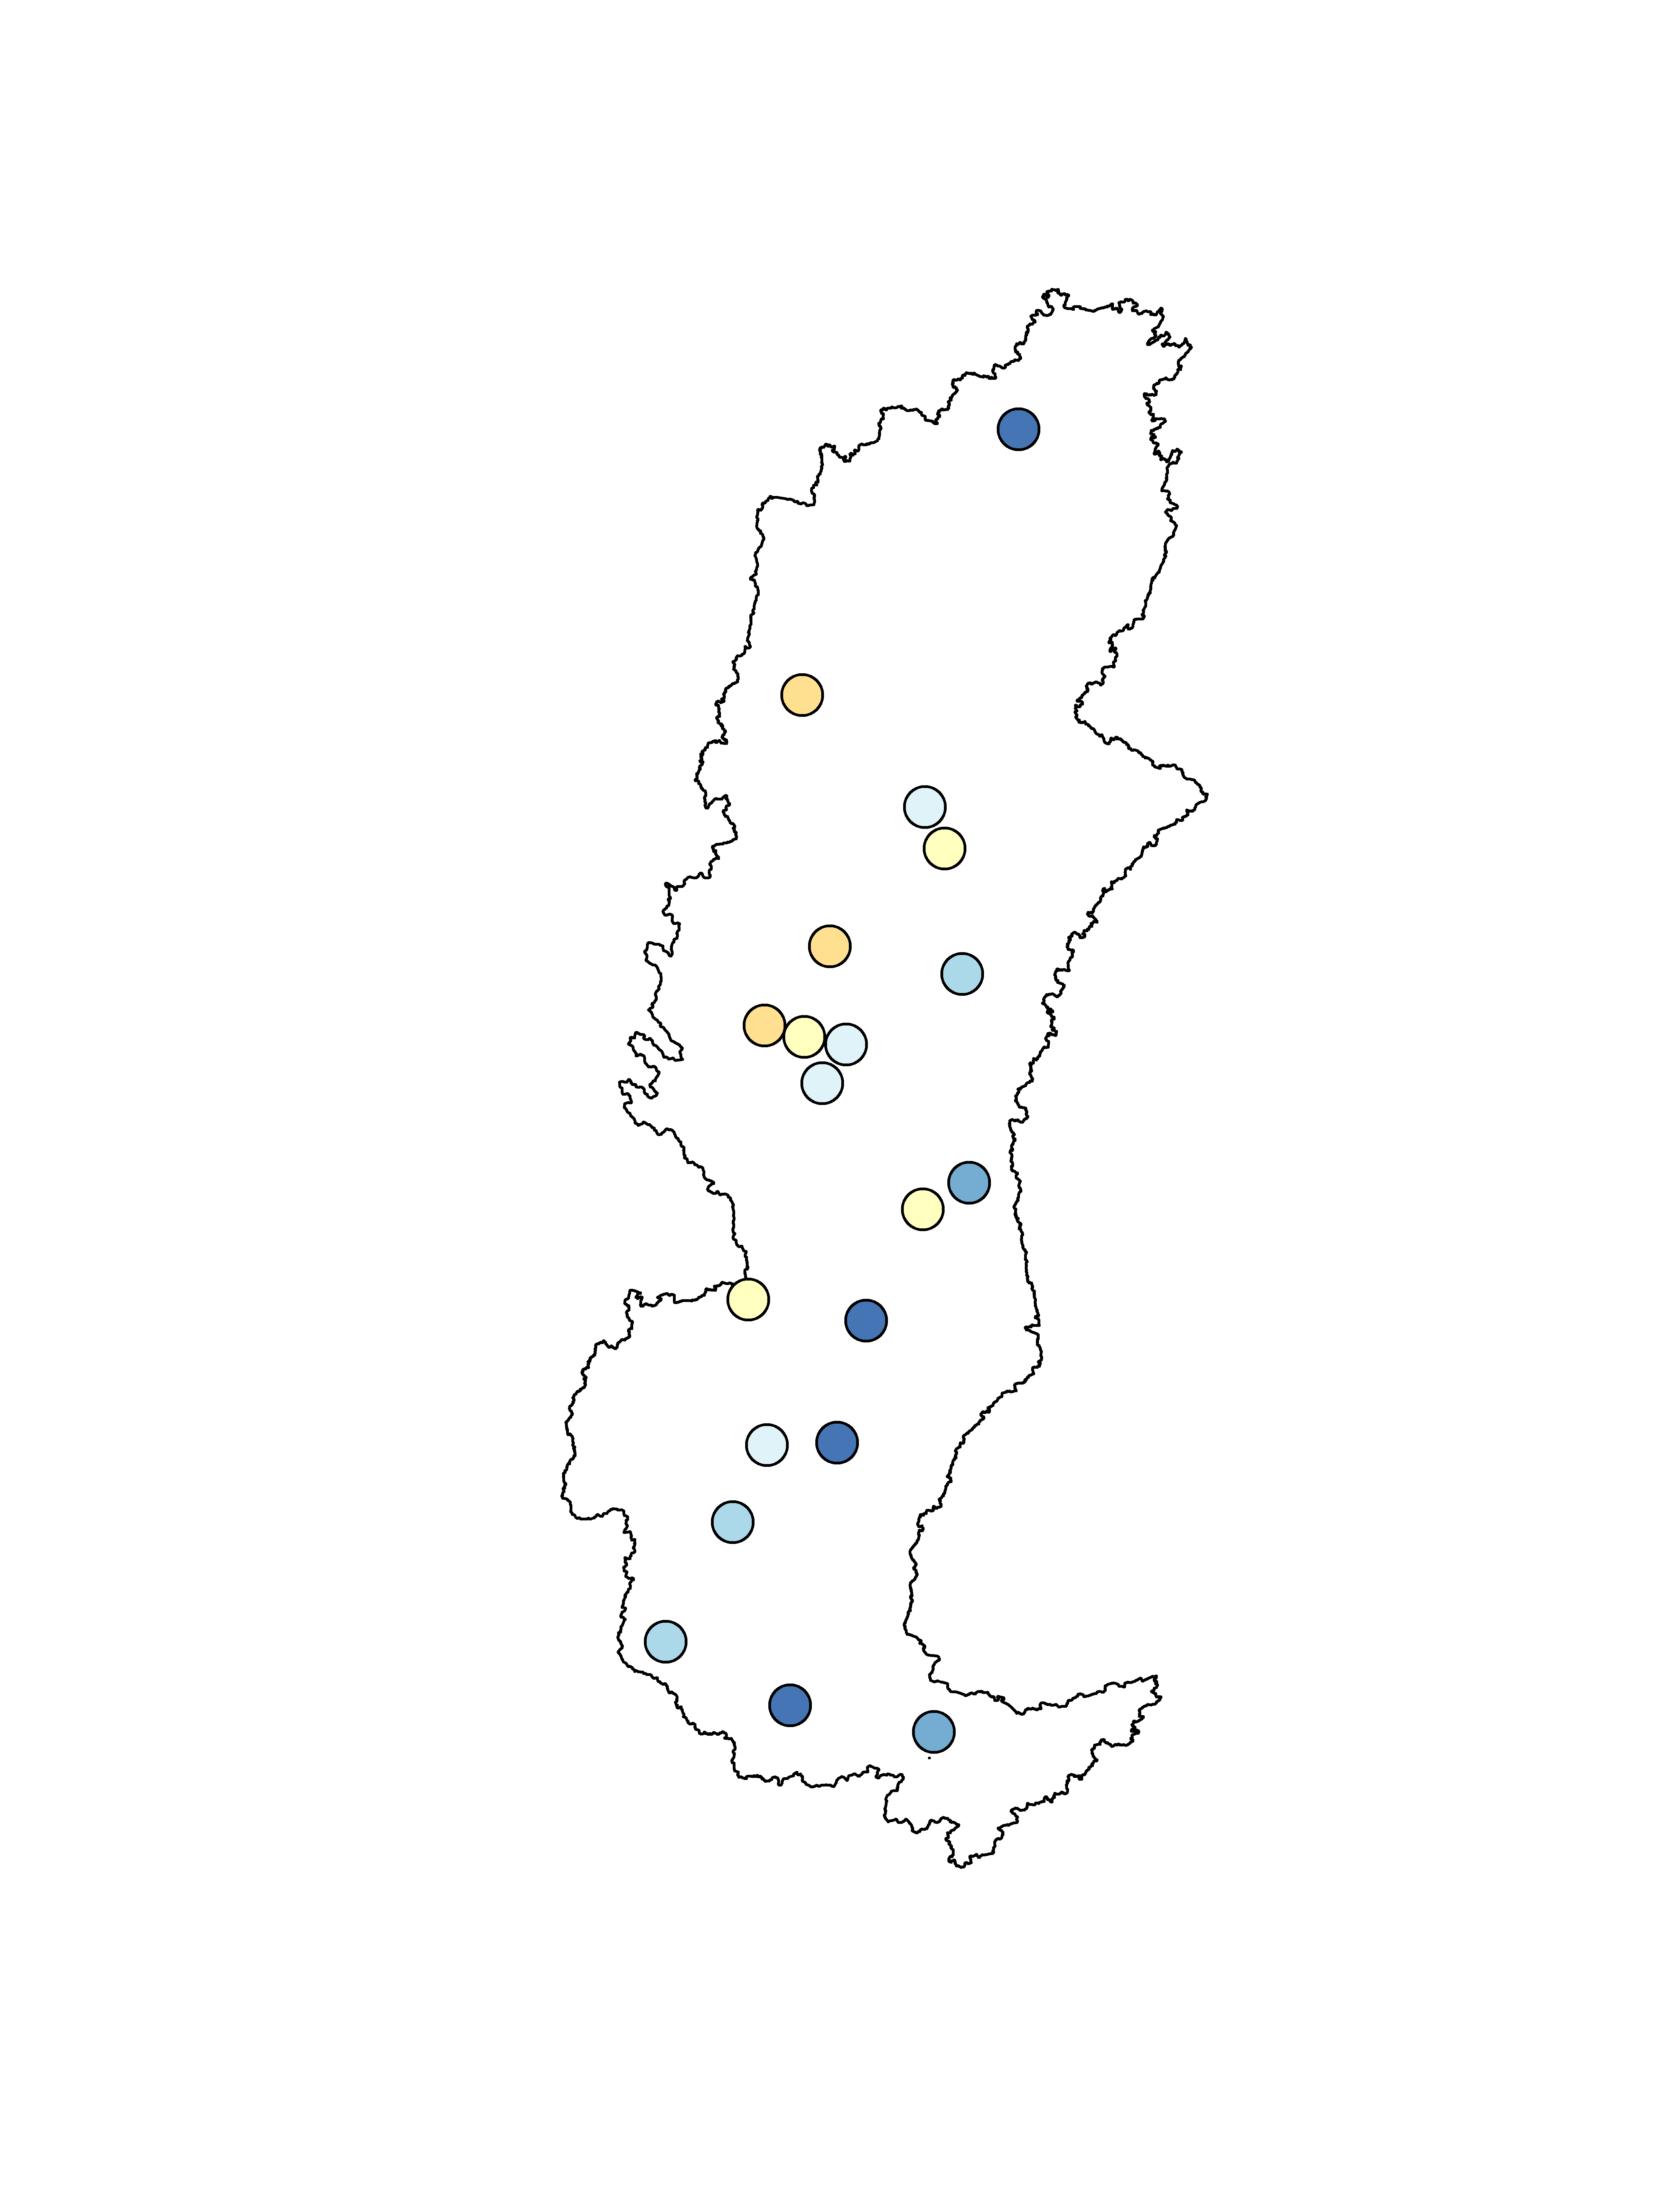
\includegraphics[trim= 4cm 2cm 1cm 2cm, clip, scale = 0.35]{./img/nashsut_harg} &
			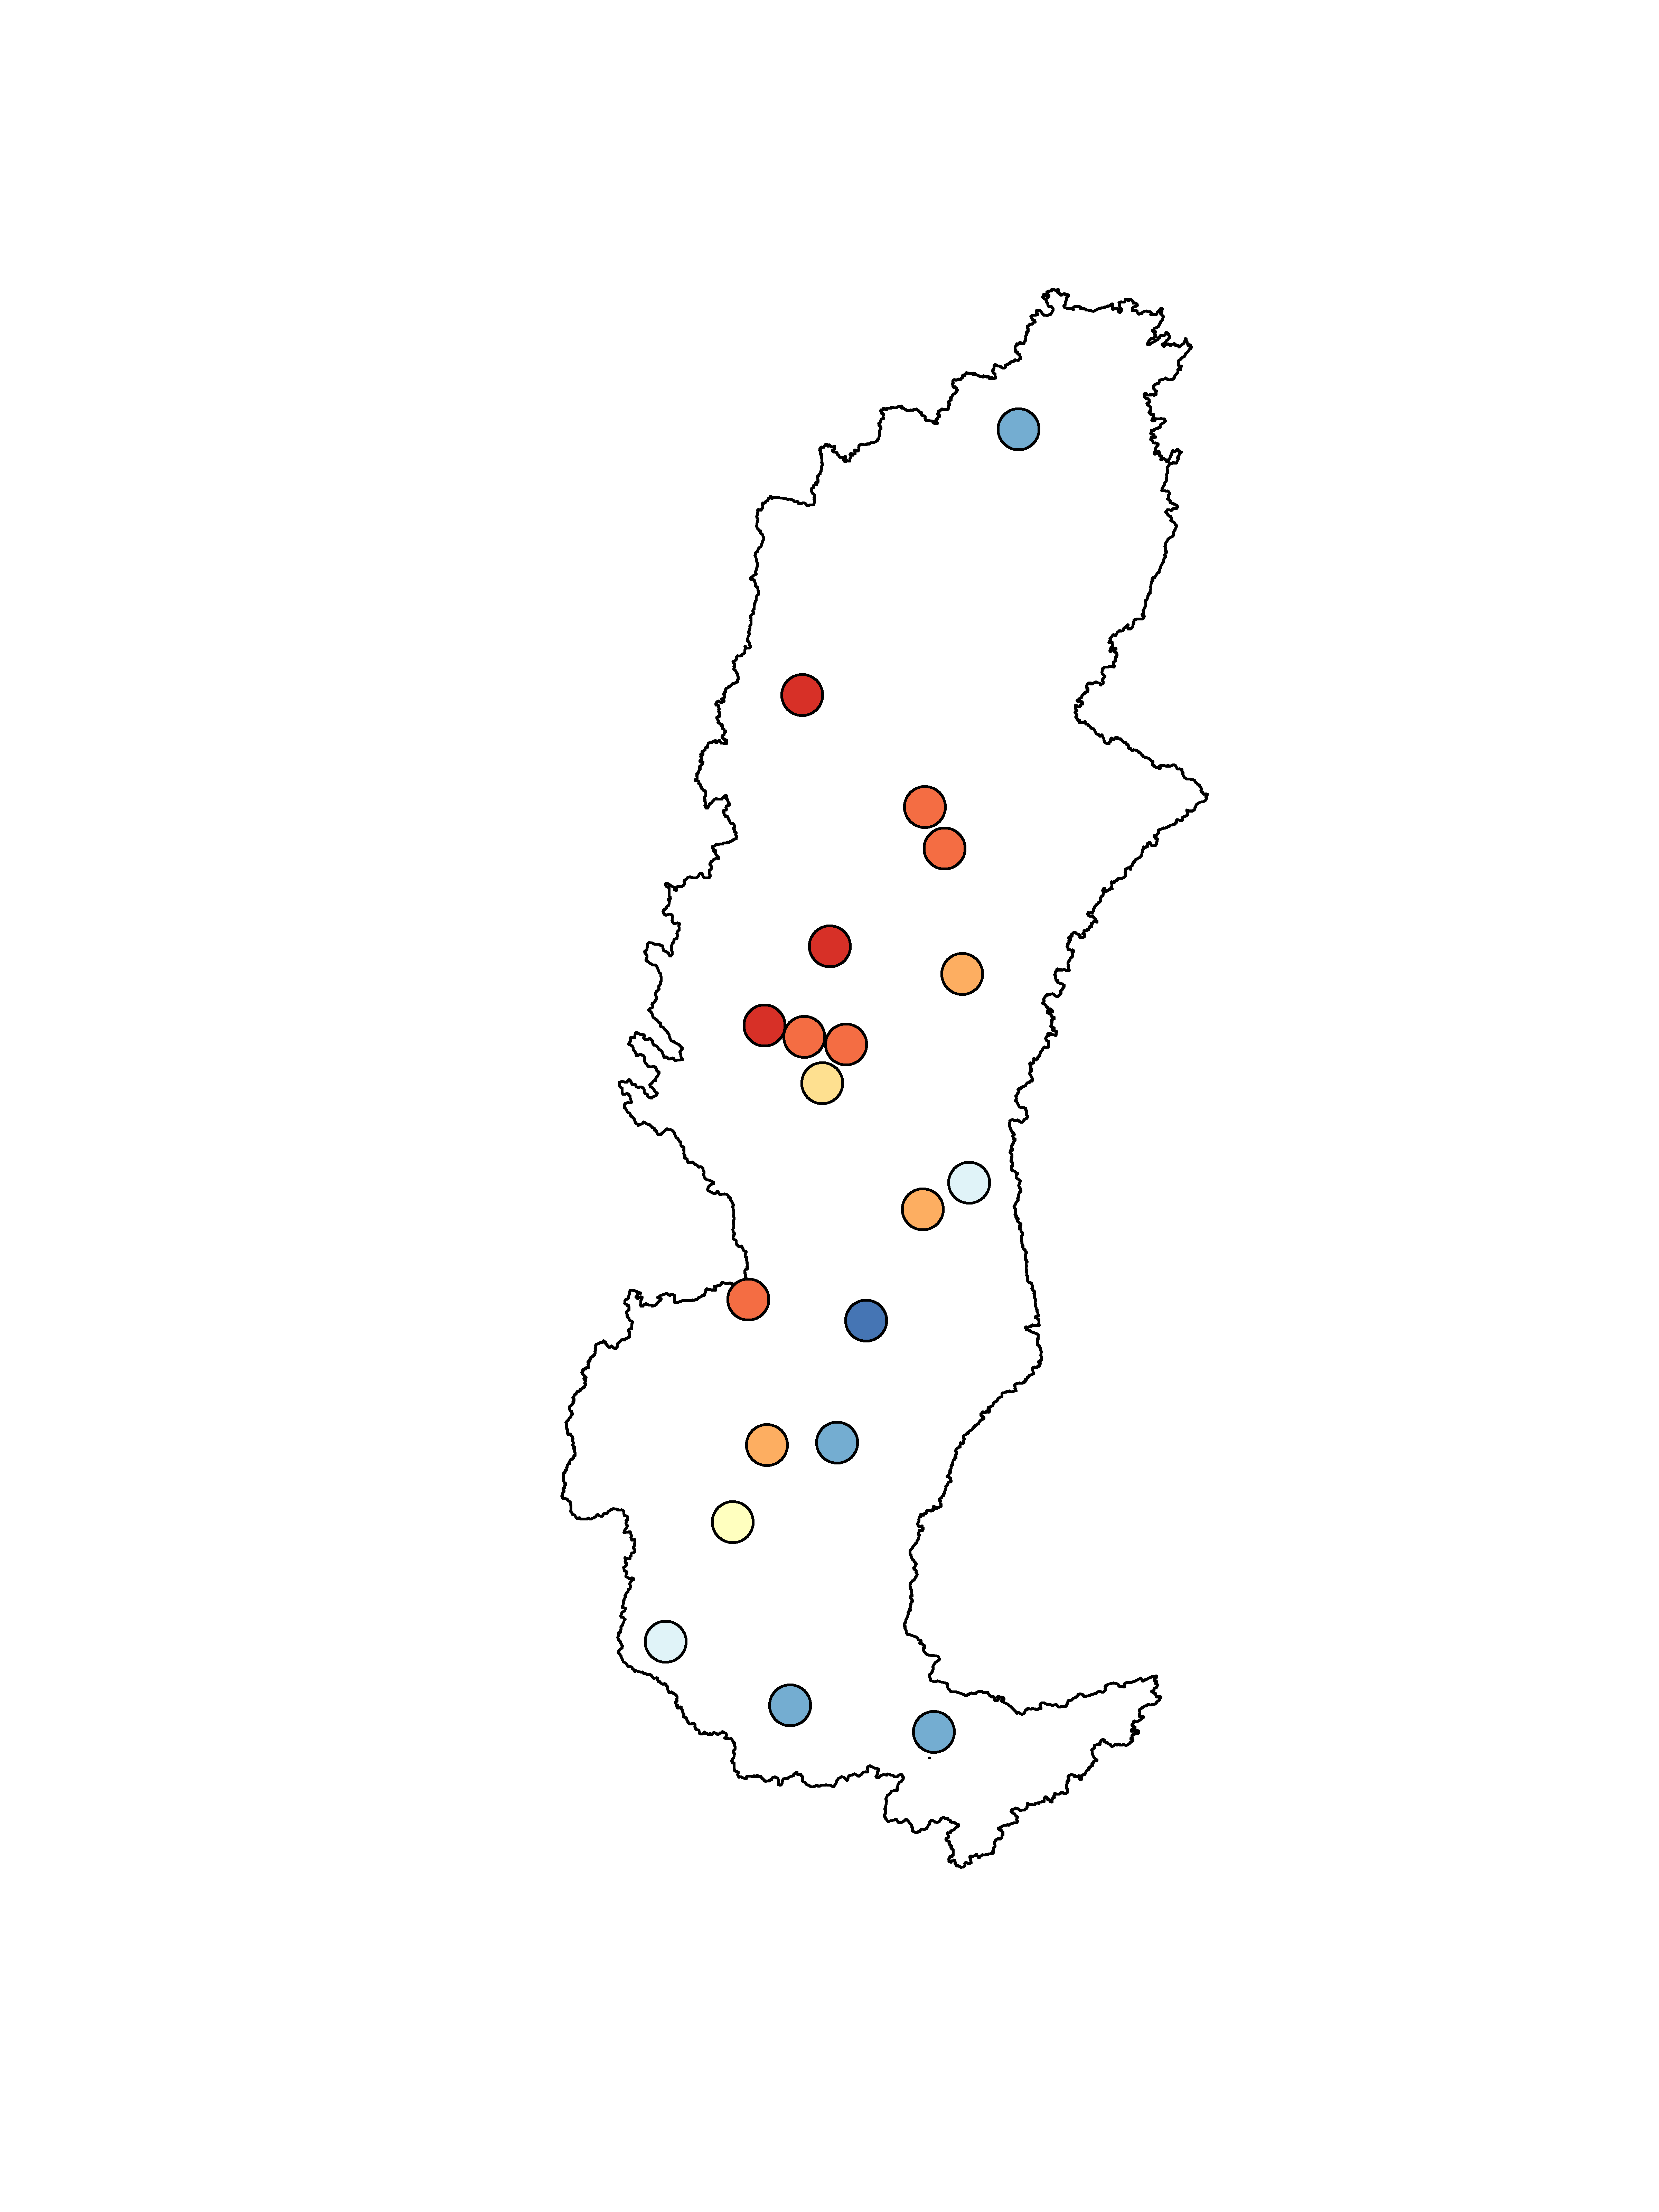
\includegraphics[trim= 4cm 2cm 1cm 2cm, clip, scale = 0.35]{./img/nashsut_penman} &
				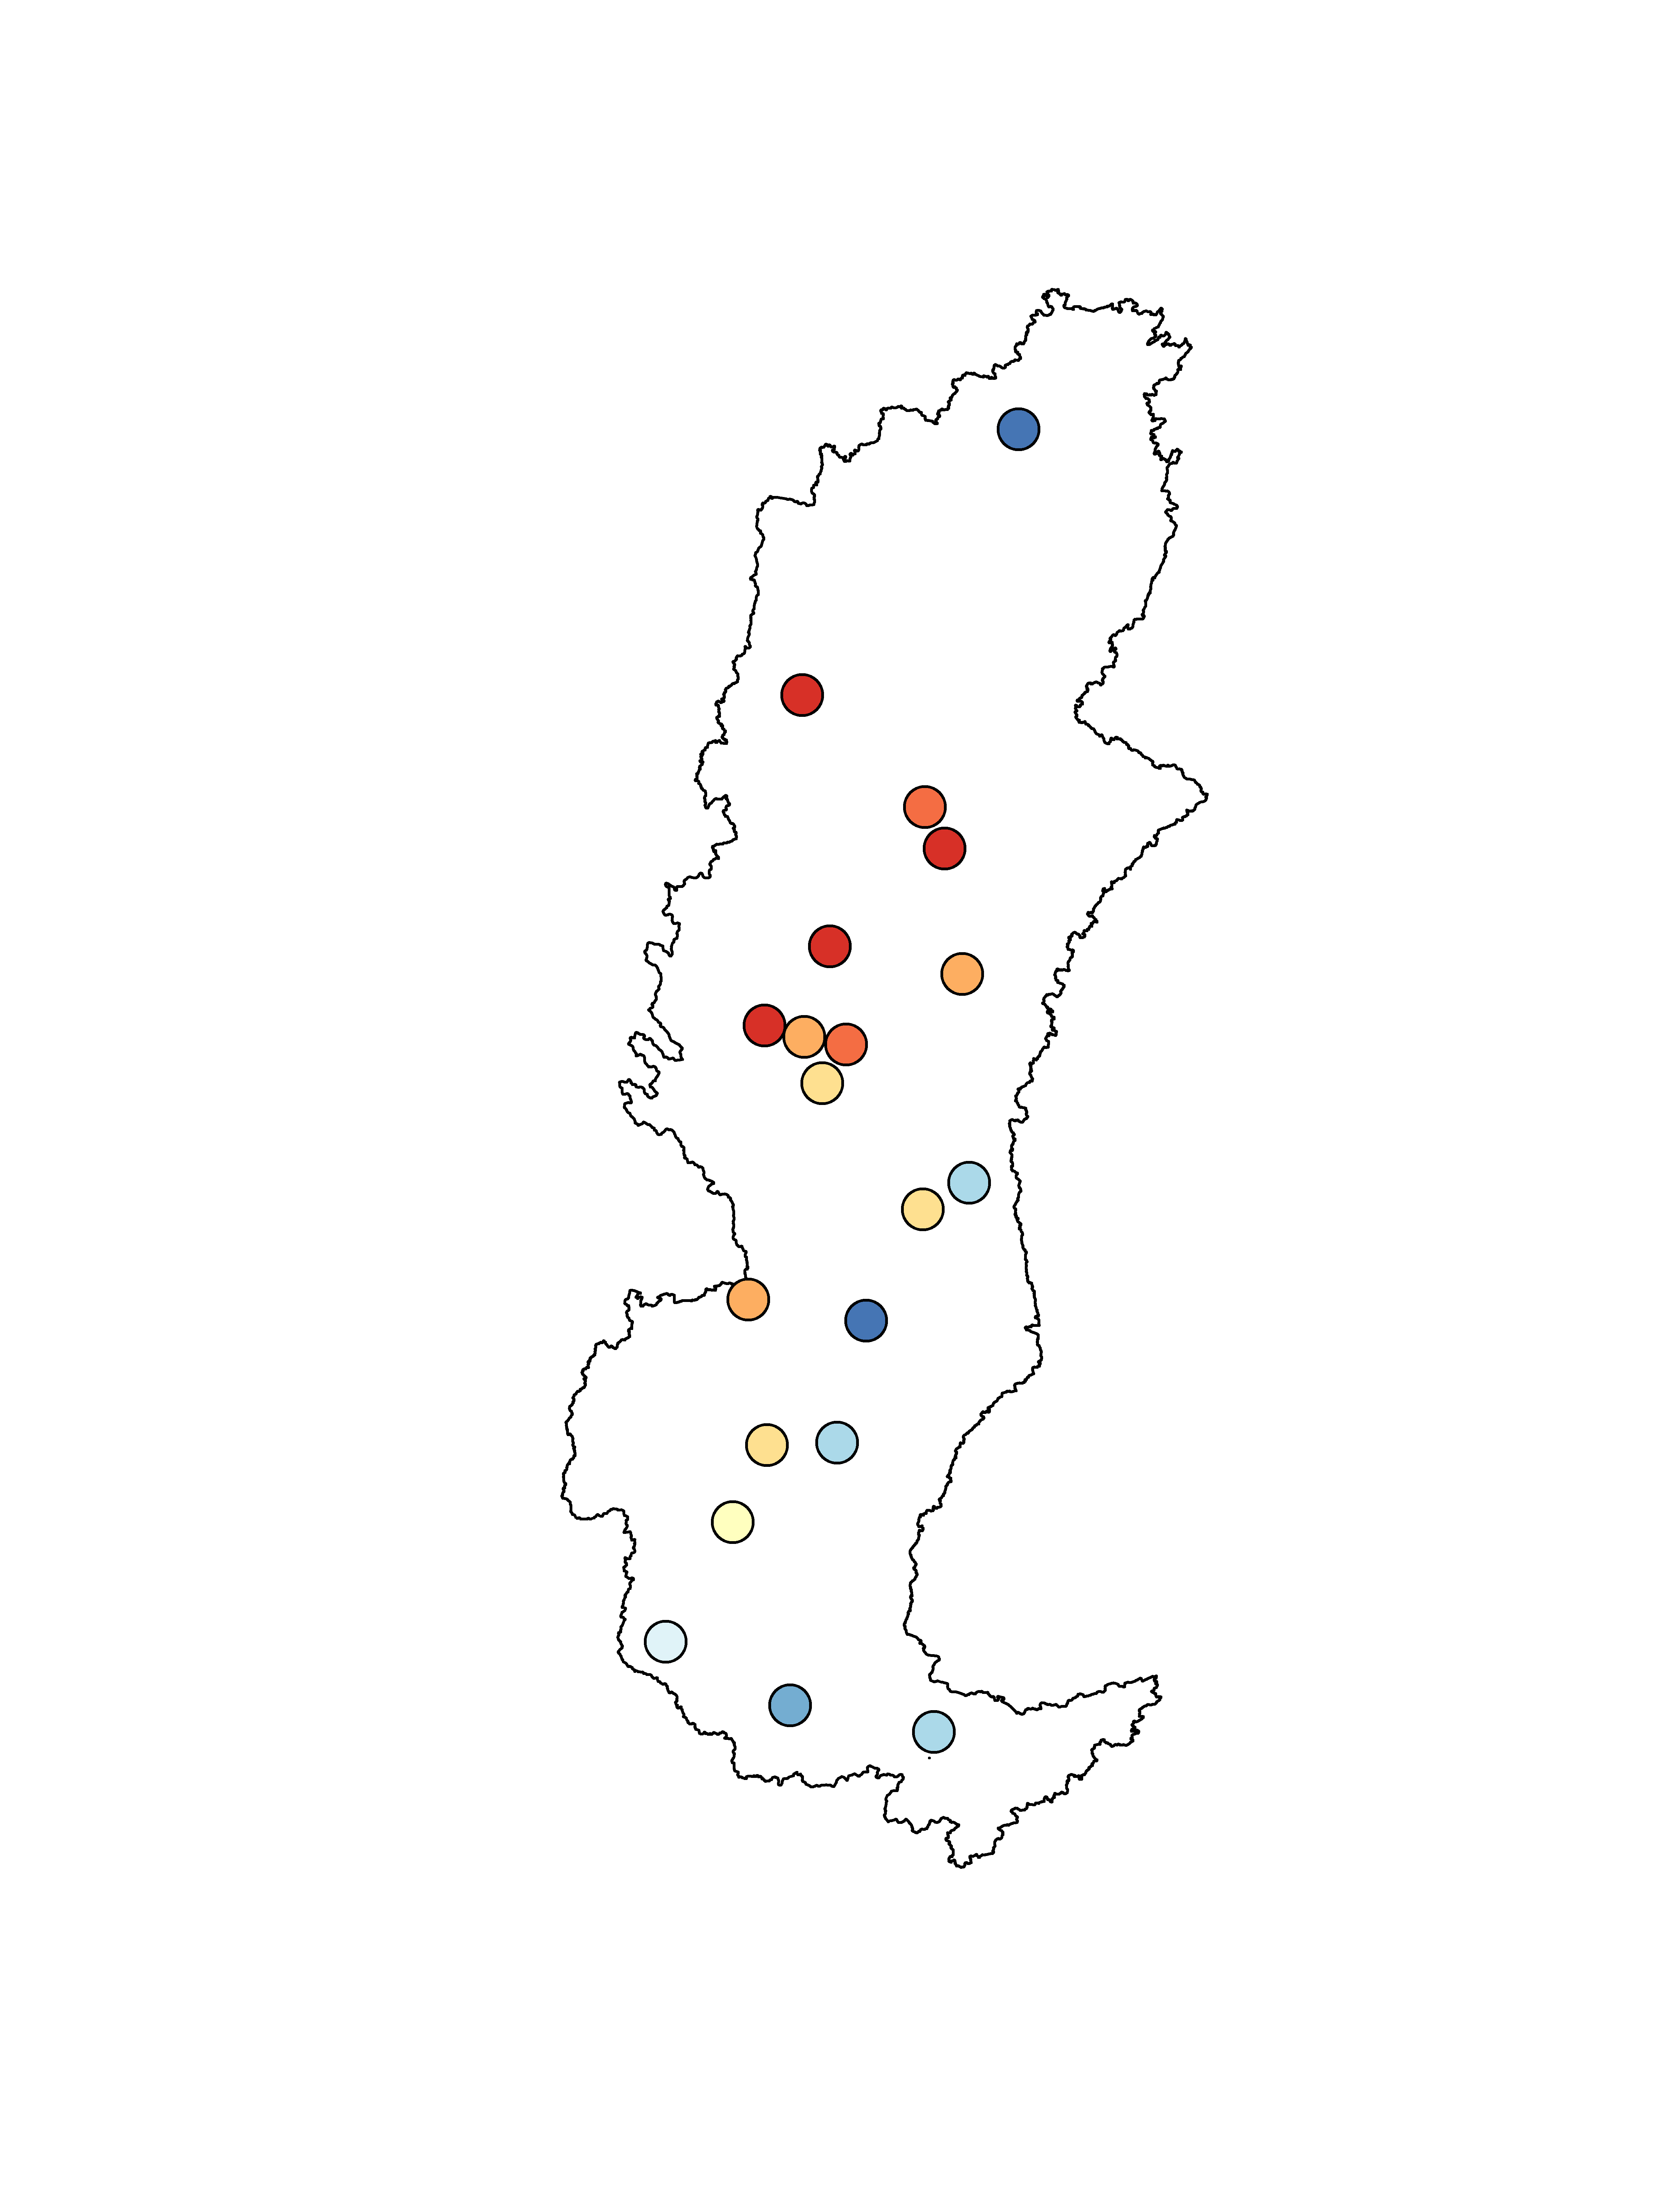
\includegraphics[trim= 4cm 2cm 1cm 2cm, clip, scale = 0.35]{./img/nashsut_priestley} &
					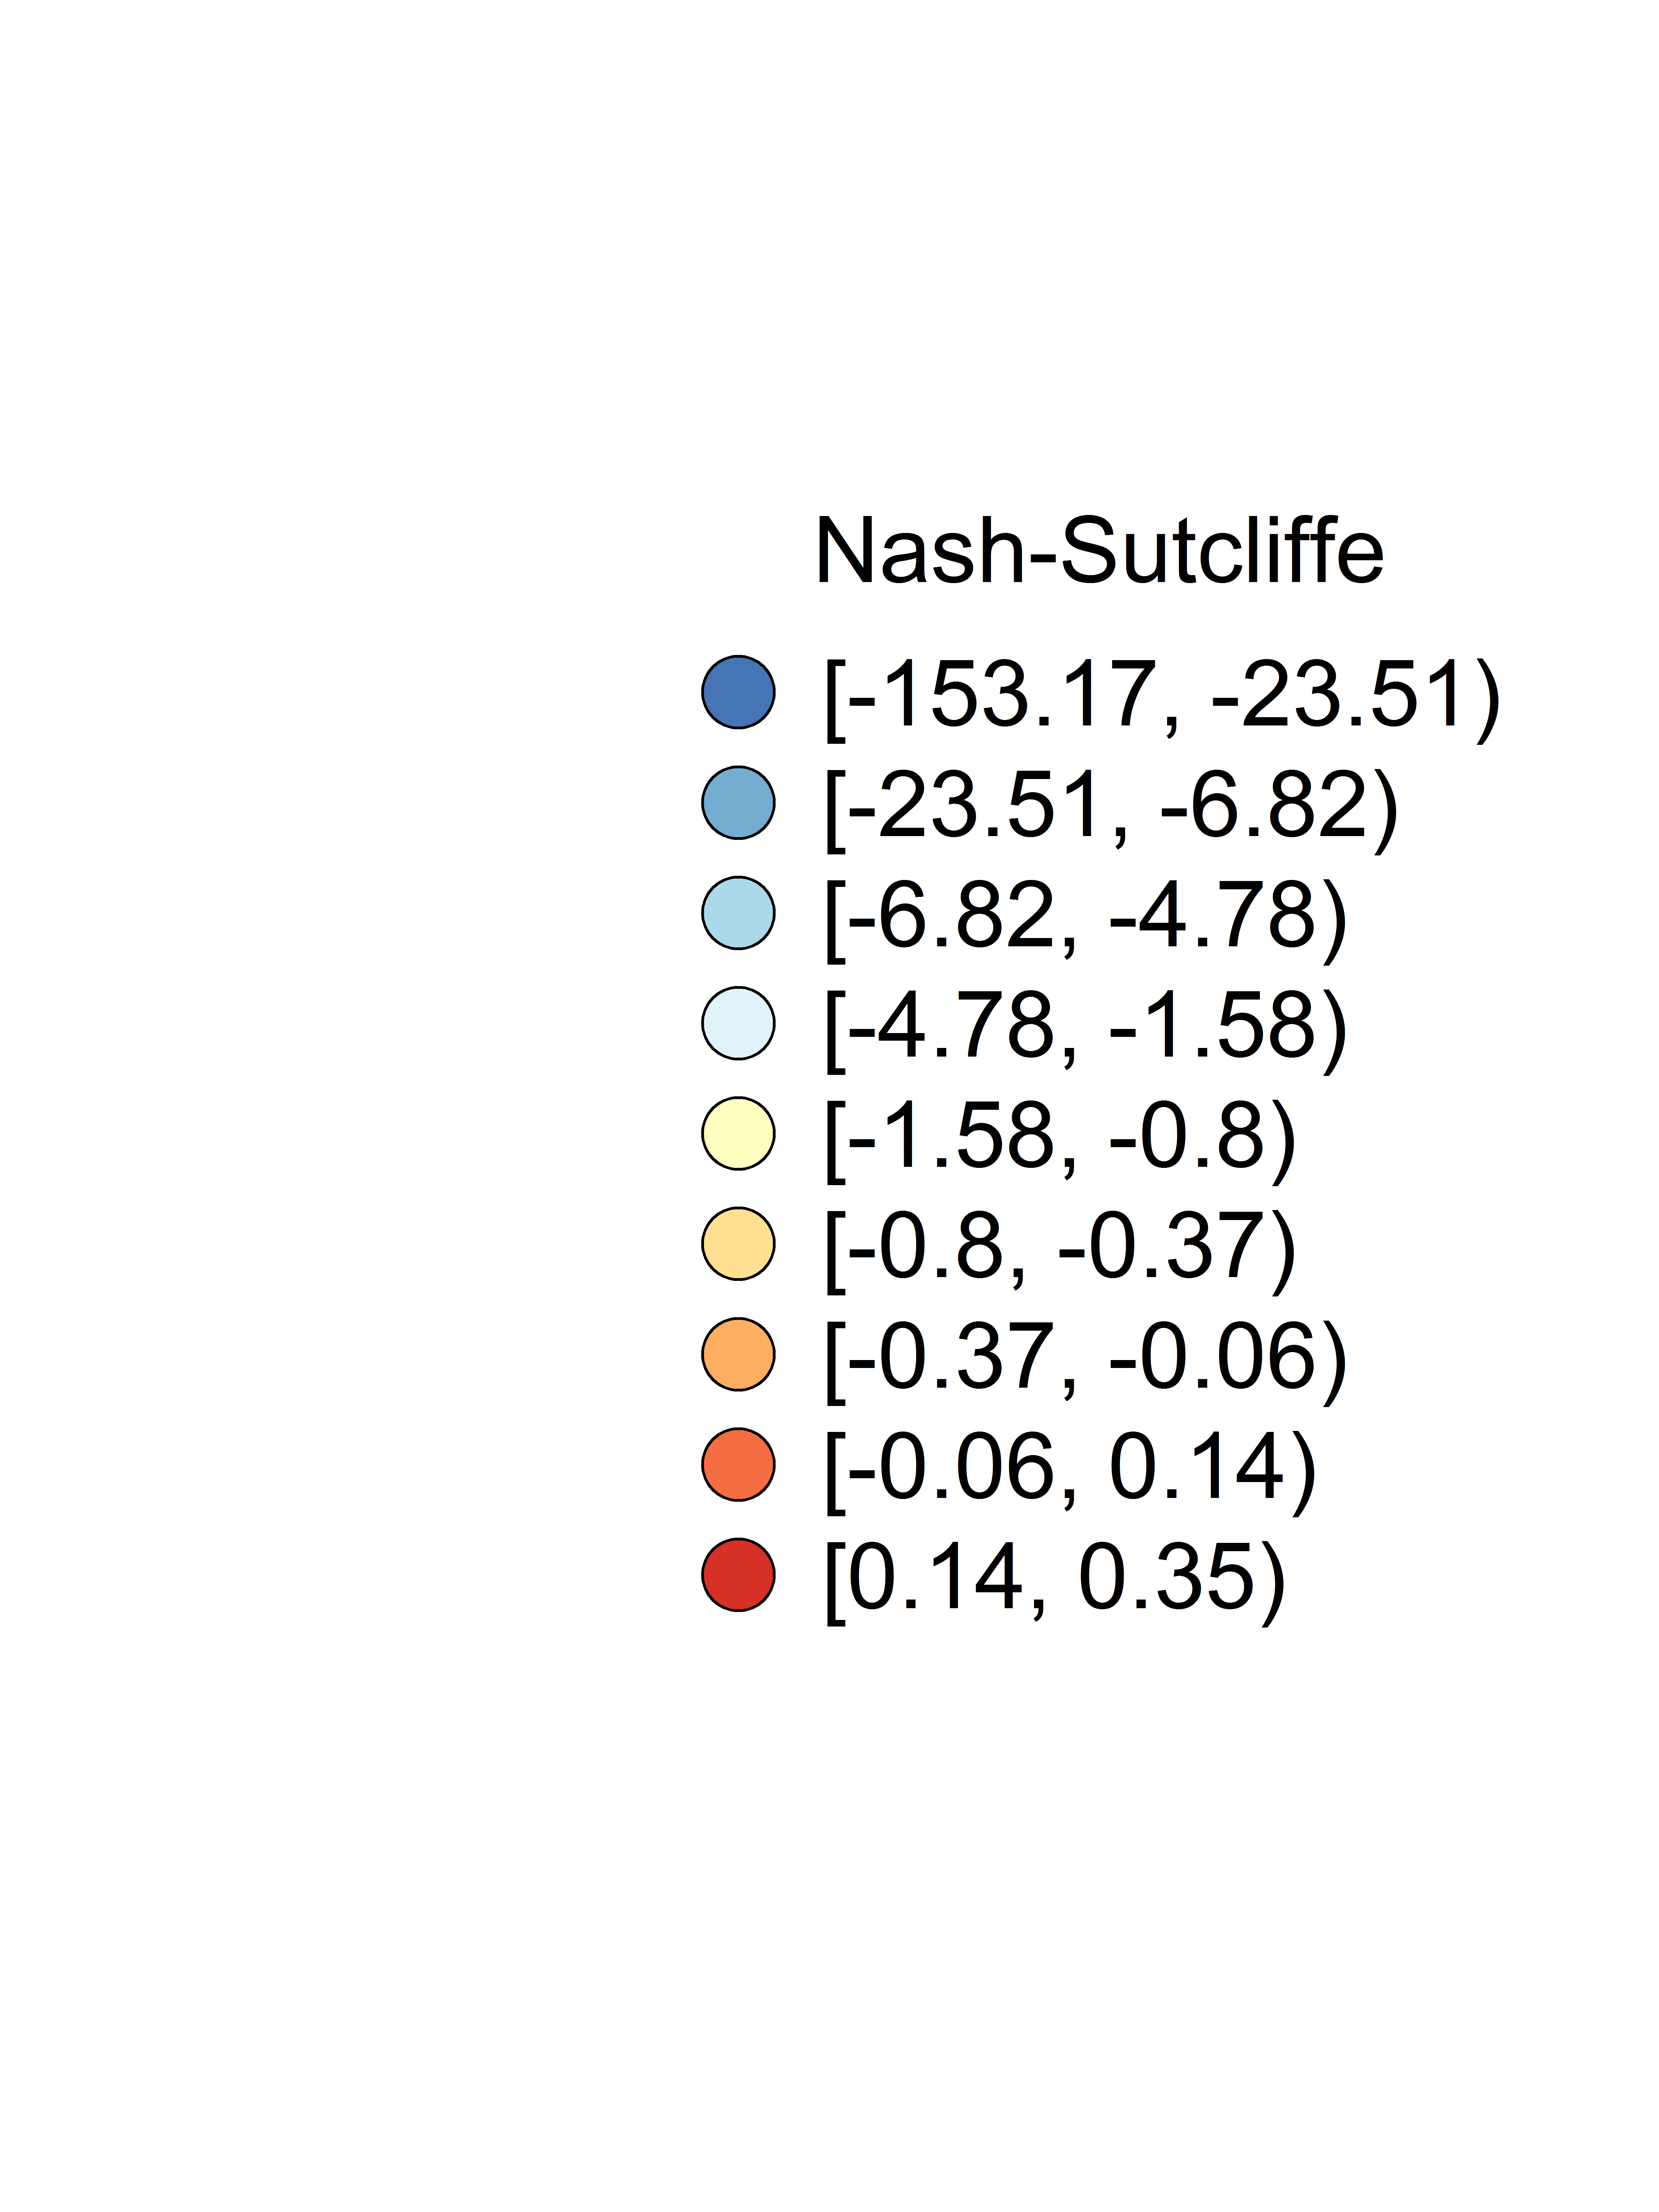
\includegraphics[trim= 5cm 2cm 0cm 3cm, clip, scale = 0.3]{./img/nashsut_legend} \\			
	\end{tabular}
\end{landscape}


% \begin{landscape}
	% \begin{figure}[h!]
		% \centering
%%%%%% for pbias %%%%%%%
		% \begin{subfigure}[b]{0.3\textwidth}
			% 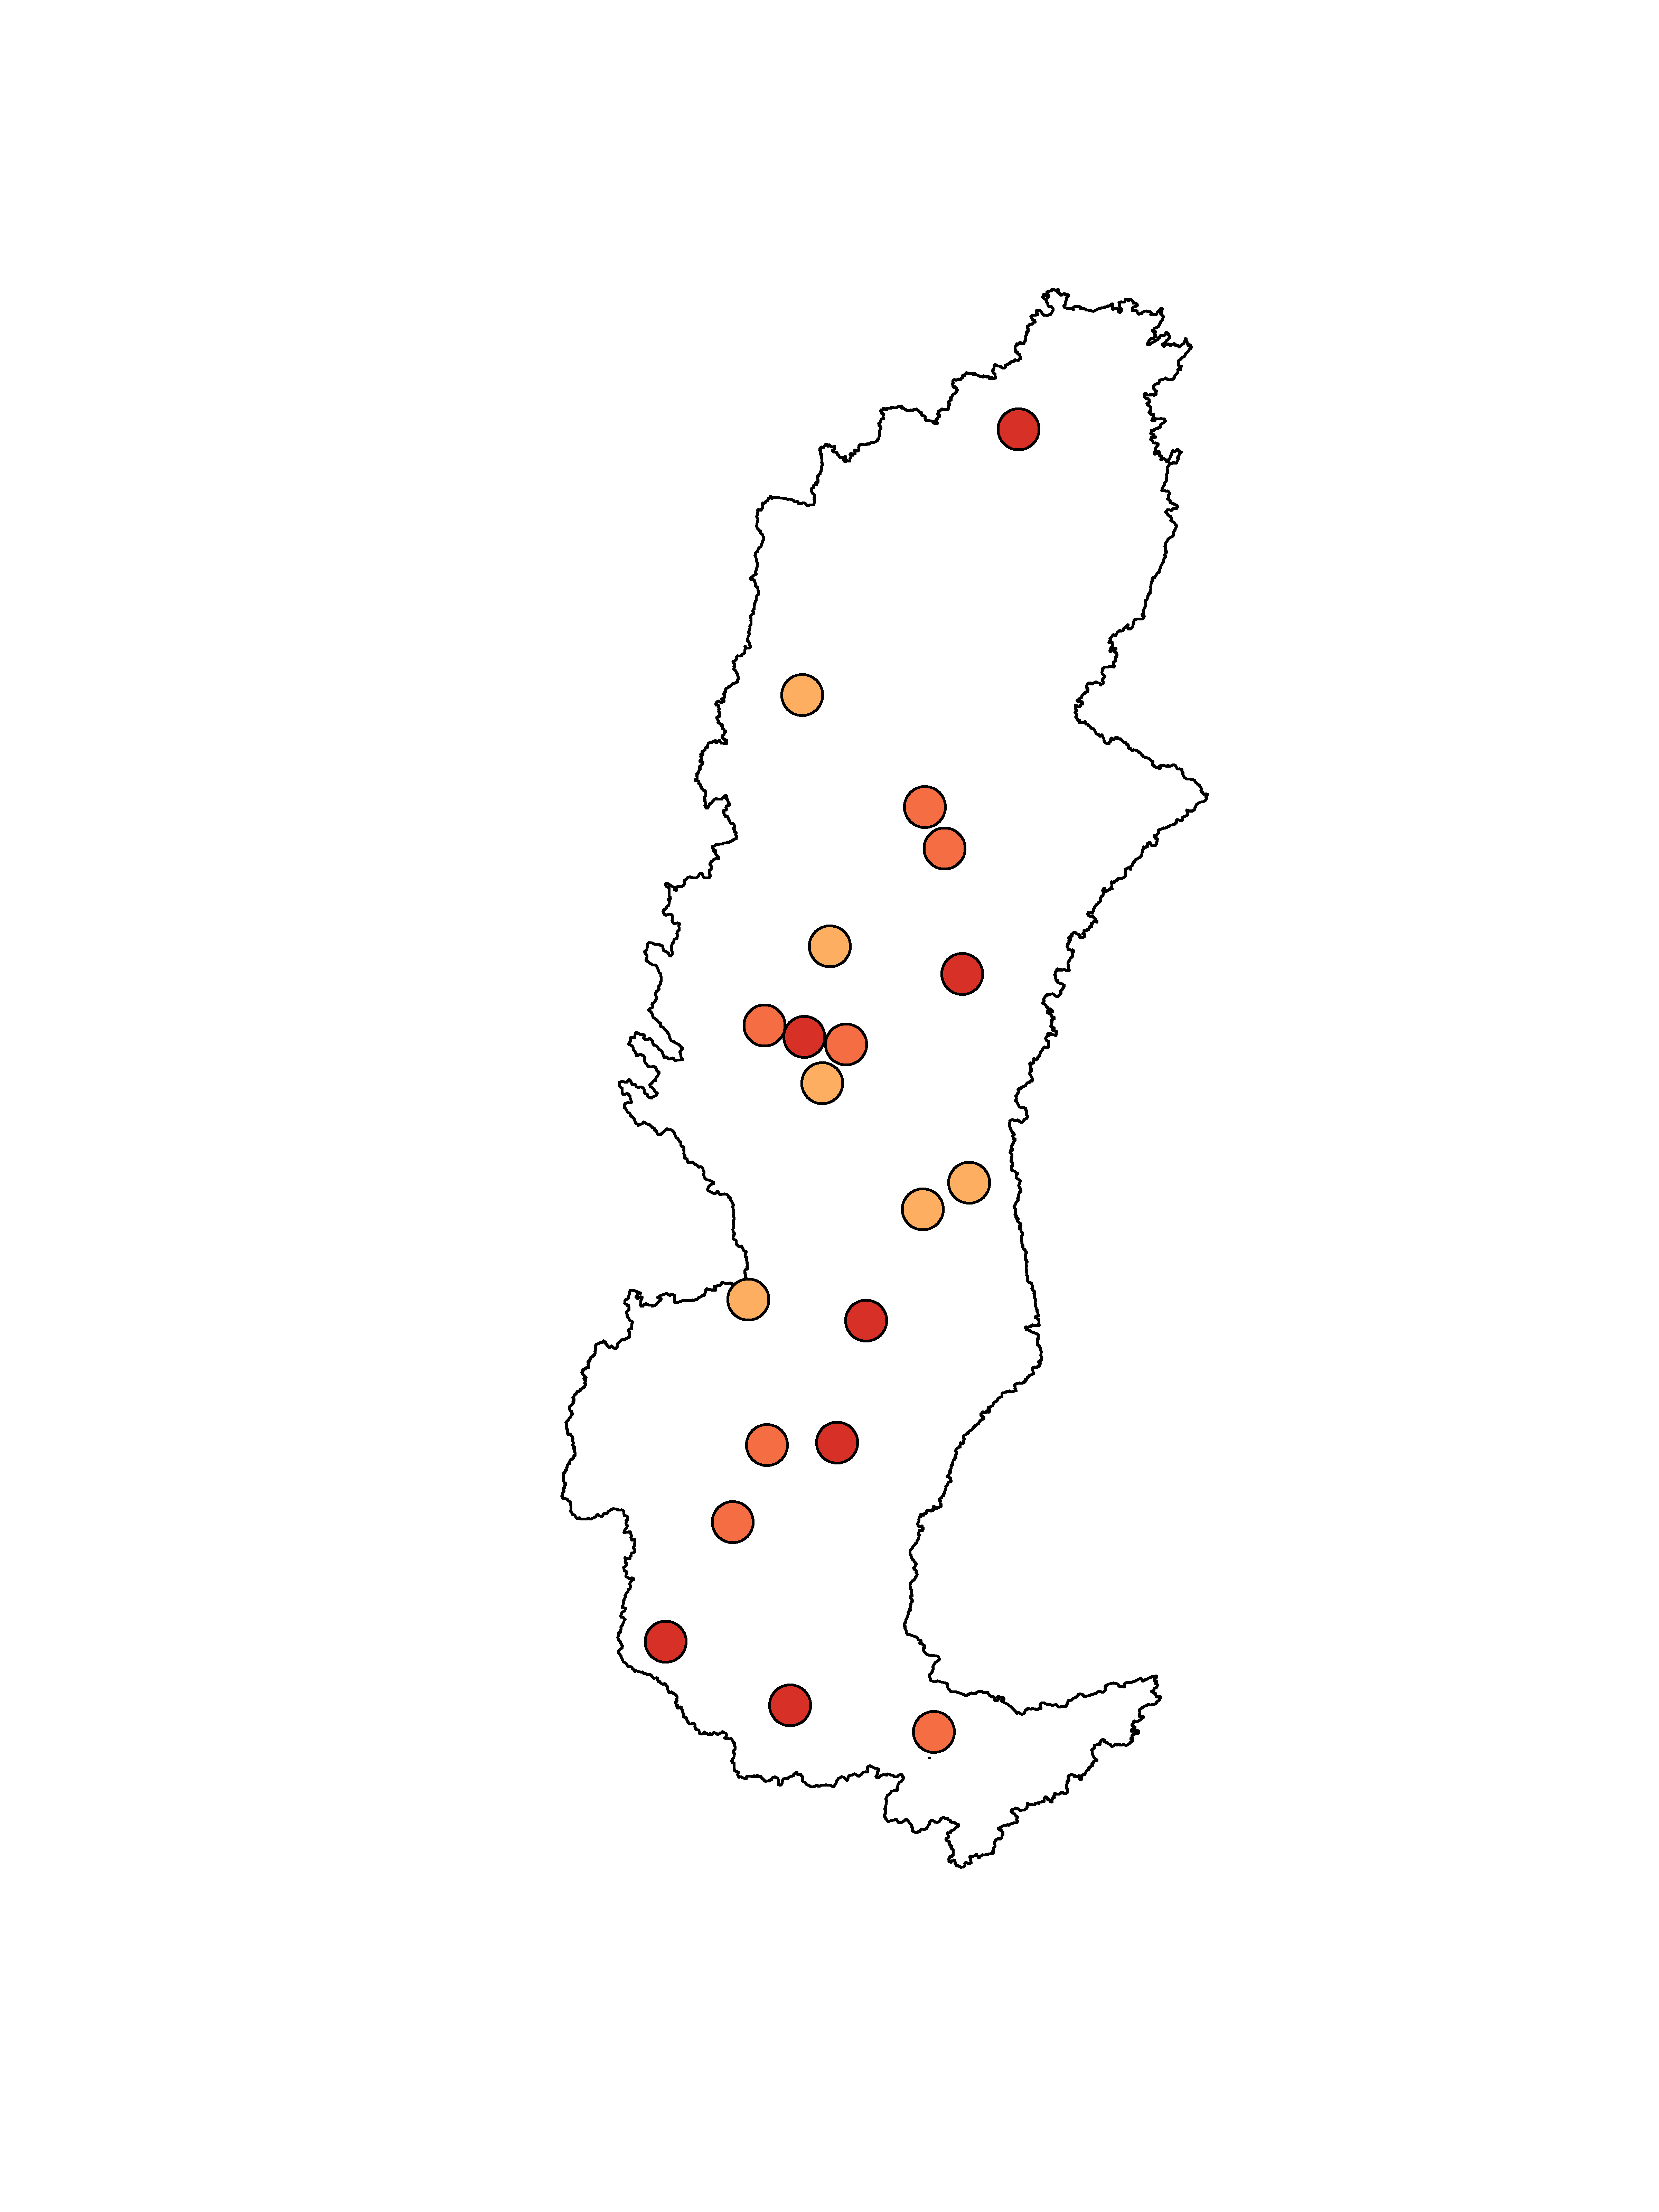
\includegraphics[scale=0.2]{./img/pbias_harg}
			% \caption{}
			% \label{fig:}
		% \end{subfigure}
		
		% \begin{subfigure}[b]{0.3\textwidth}
			% 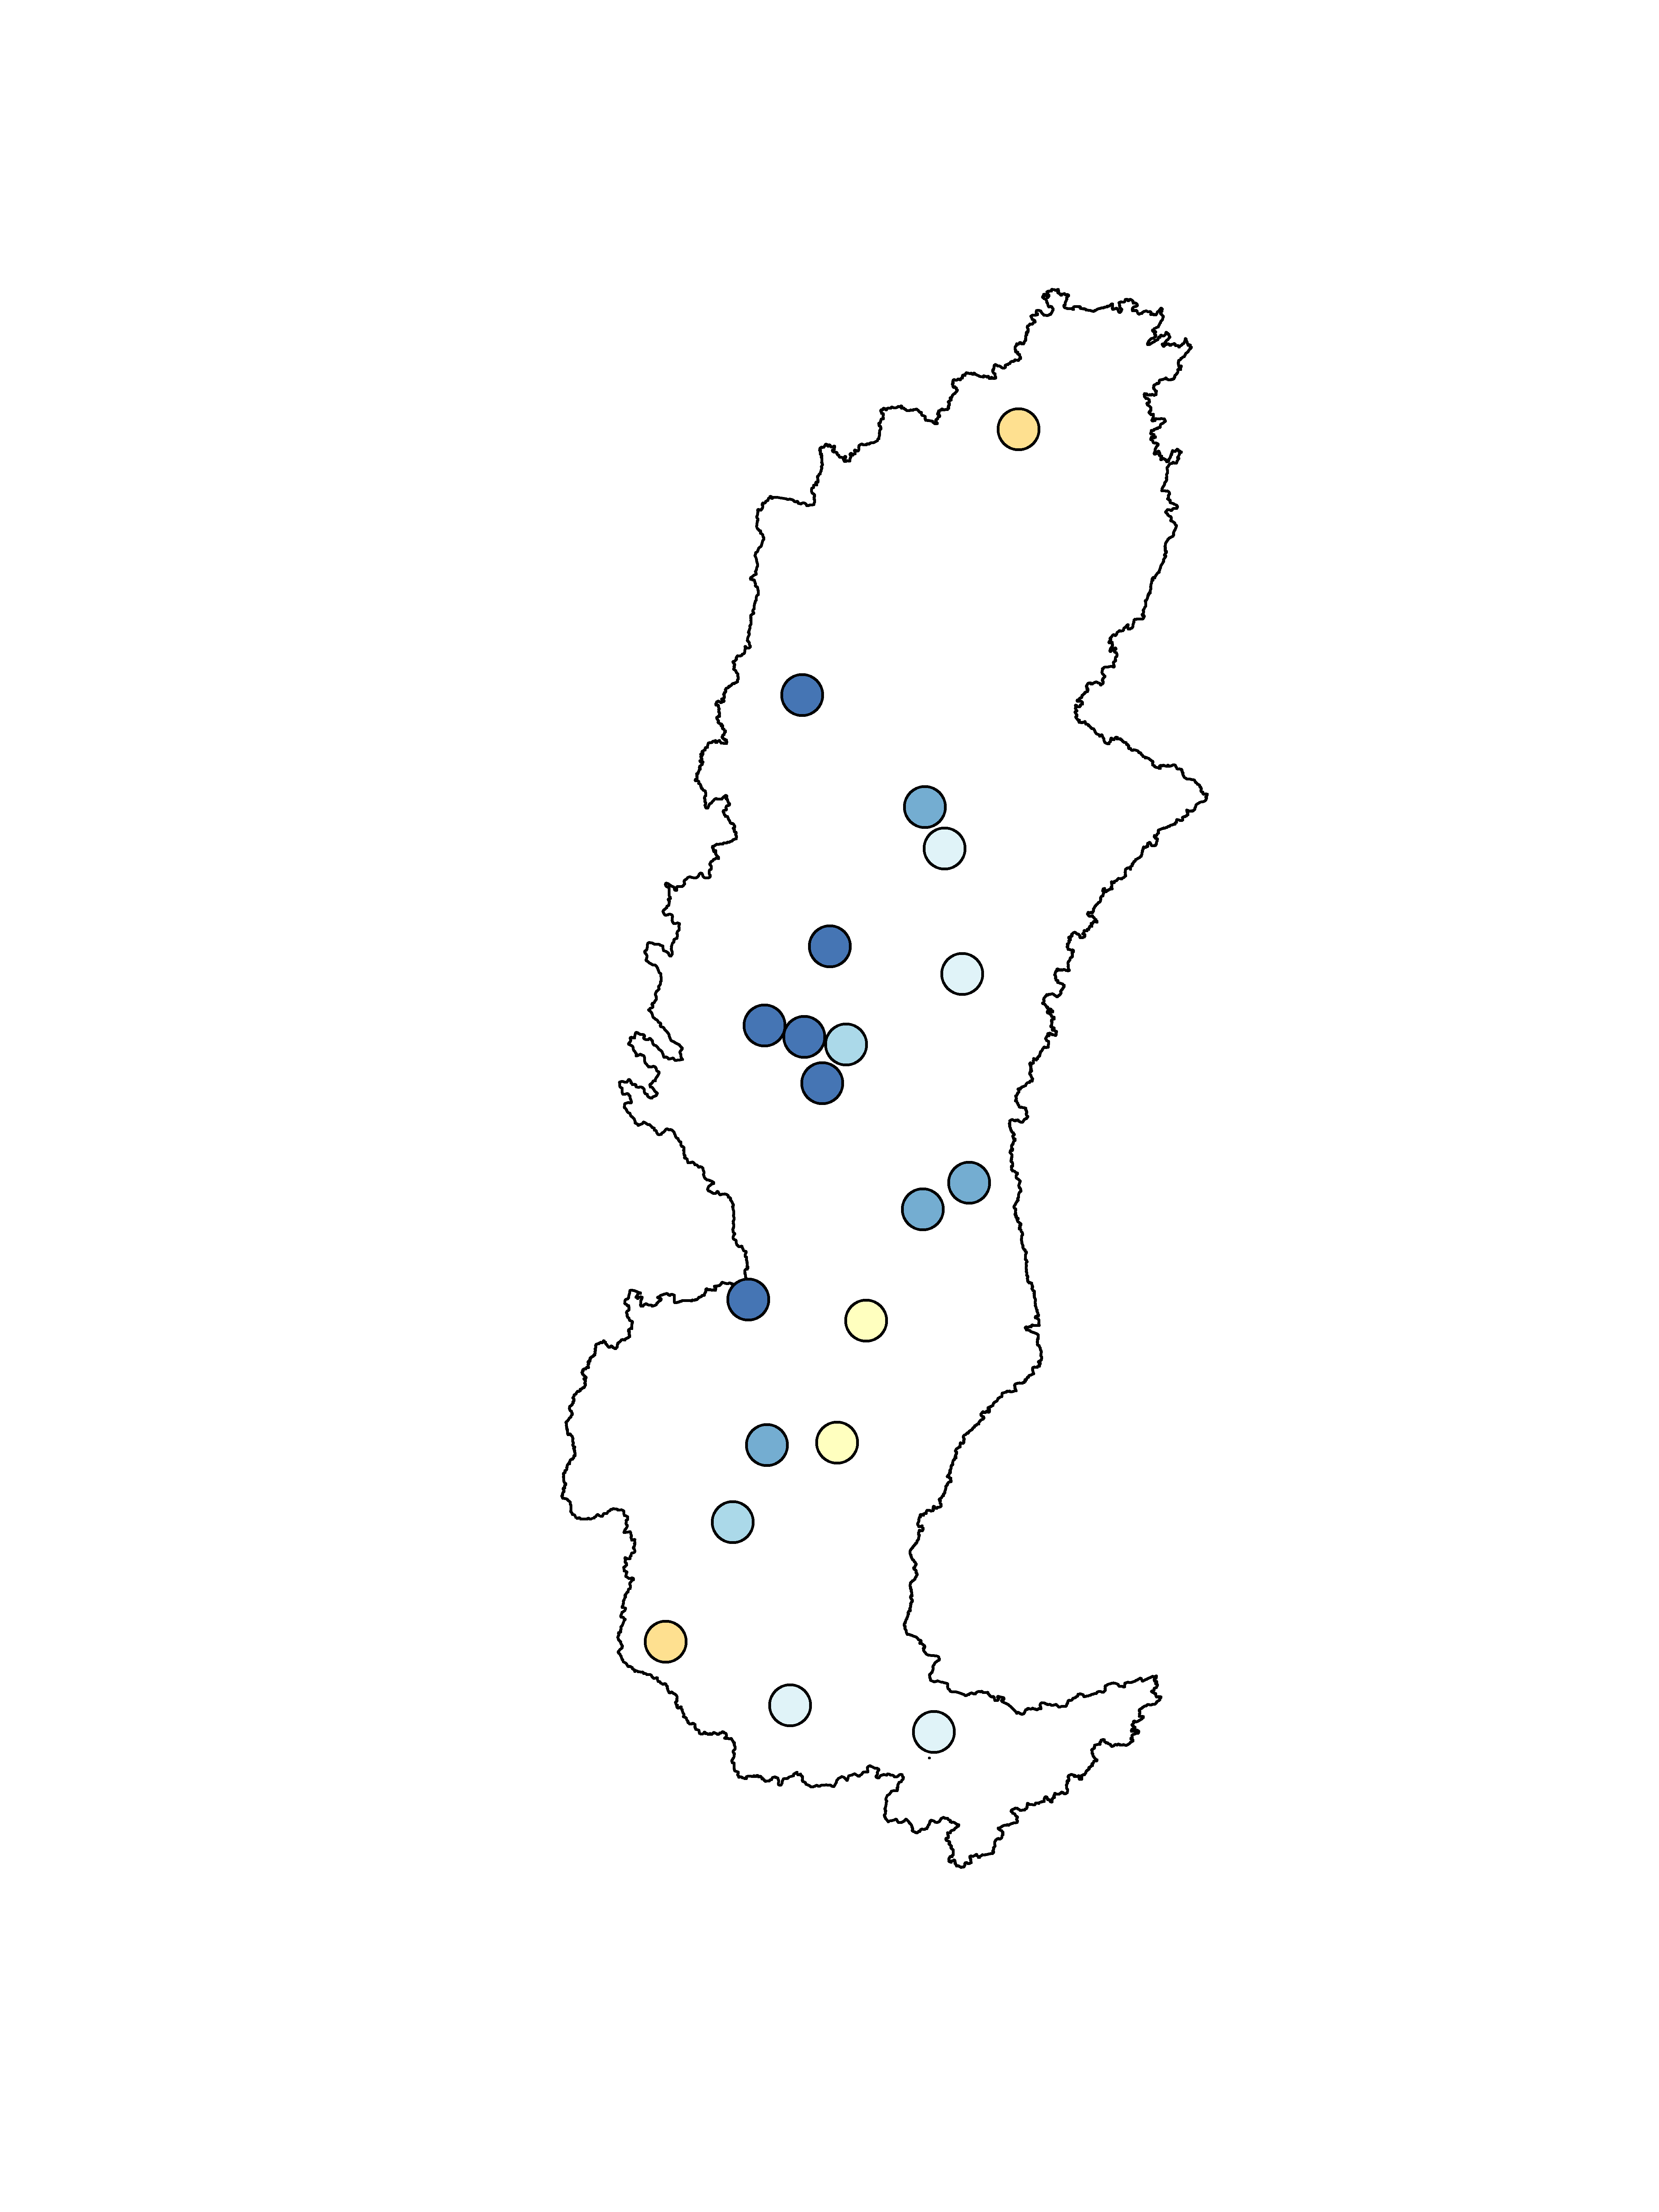
\includegraphics[scale=0.2]{./img/pbias_penman}
			% \caption{}
			% \label{fig:}
		% \end{subfigure}
		
		
		% \begin{subfigure}[b]{0.3\textwidth}
			% 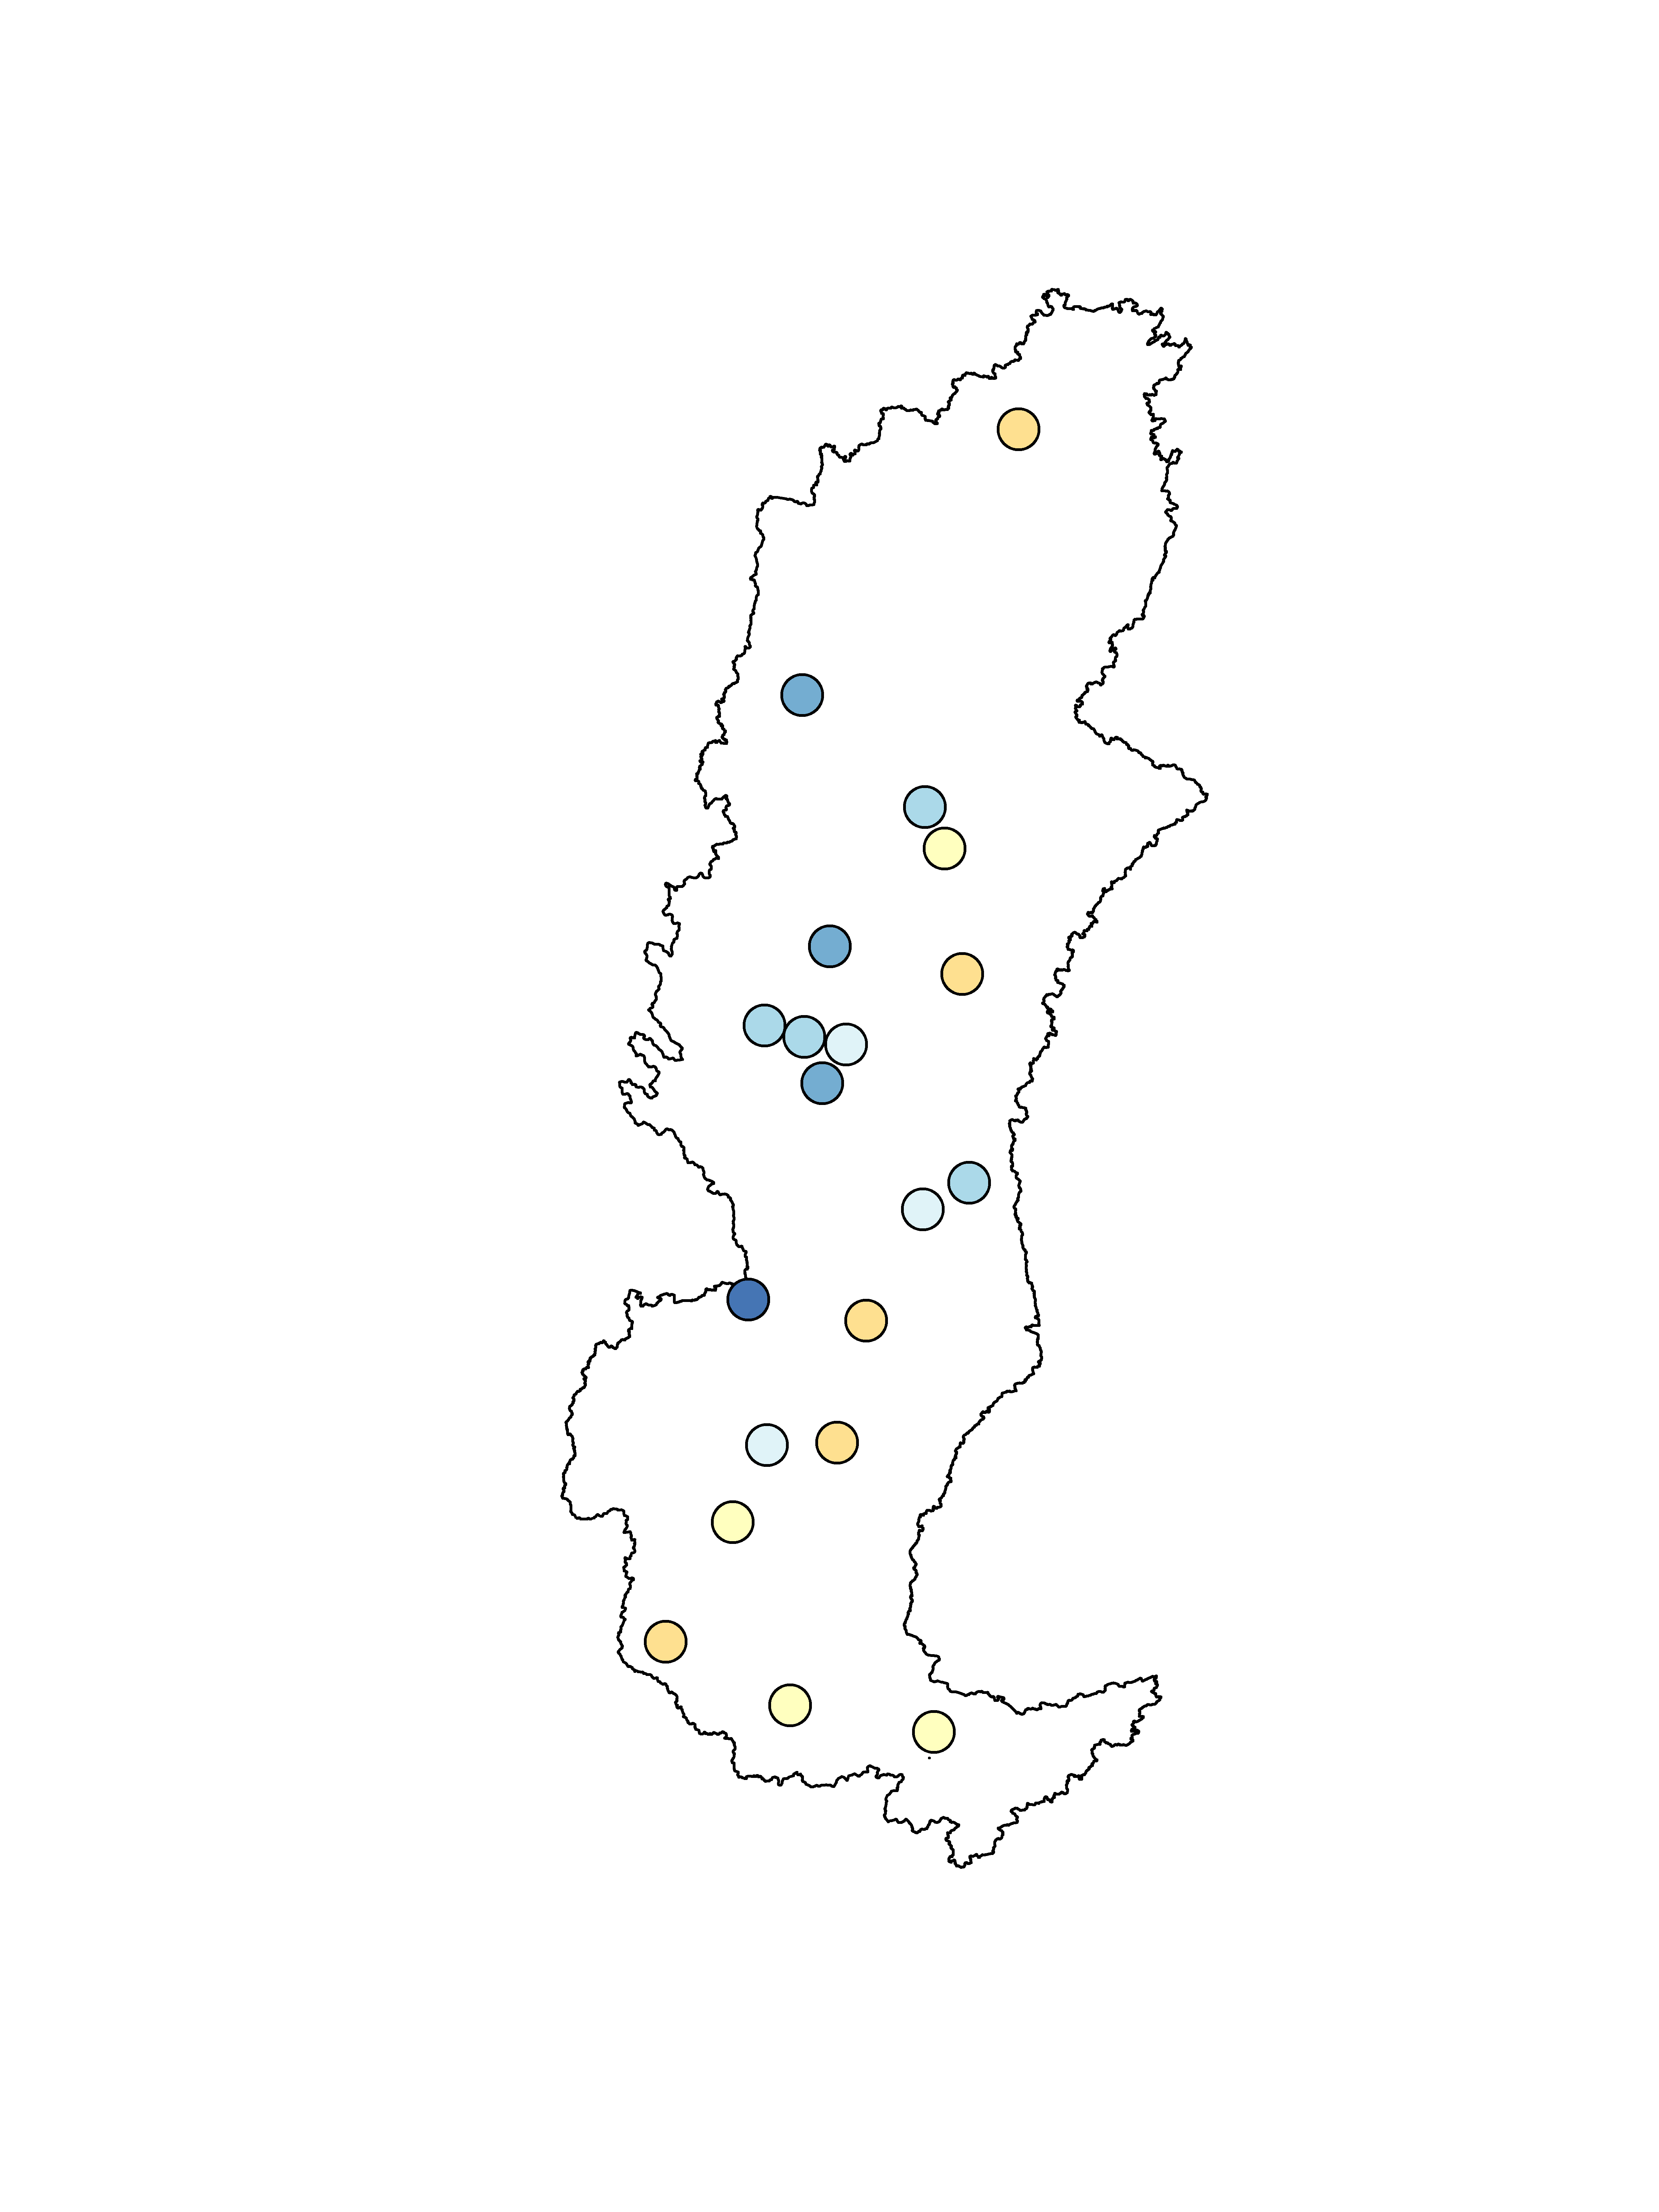
\includegraphics[scale=0.2]{./img/pbias_priestley}
			% \caption{}
			% \label{fig:}
		% \end{subfigure}
%%		legend
		% \begin{subfigure}[b]{0.1\textwidth}
			% 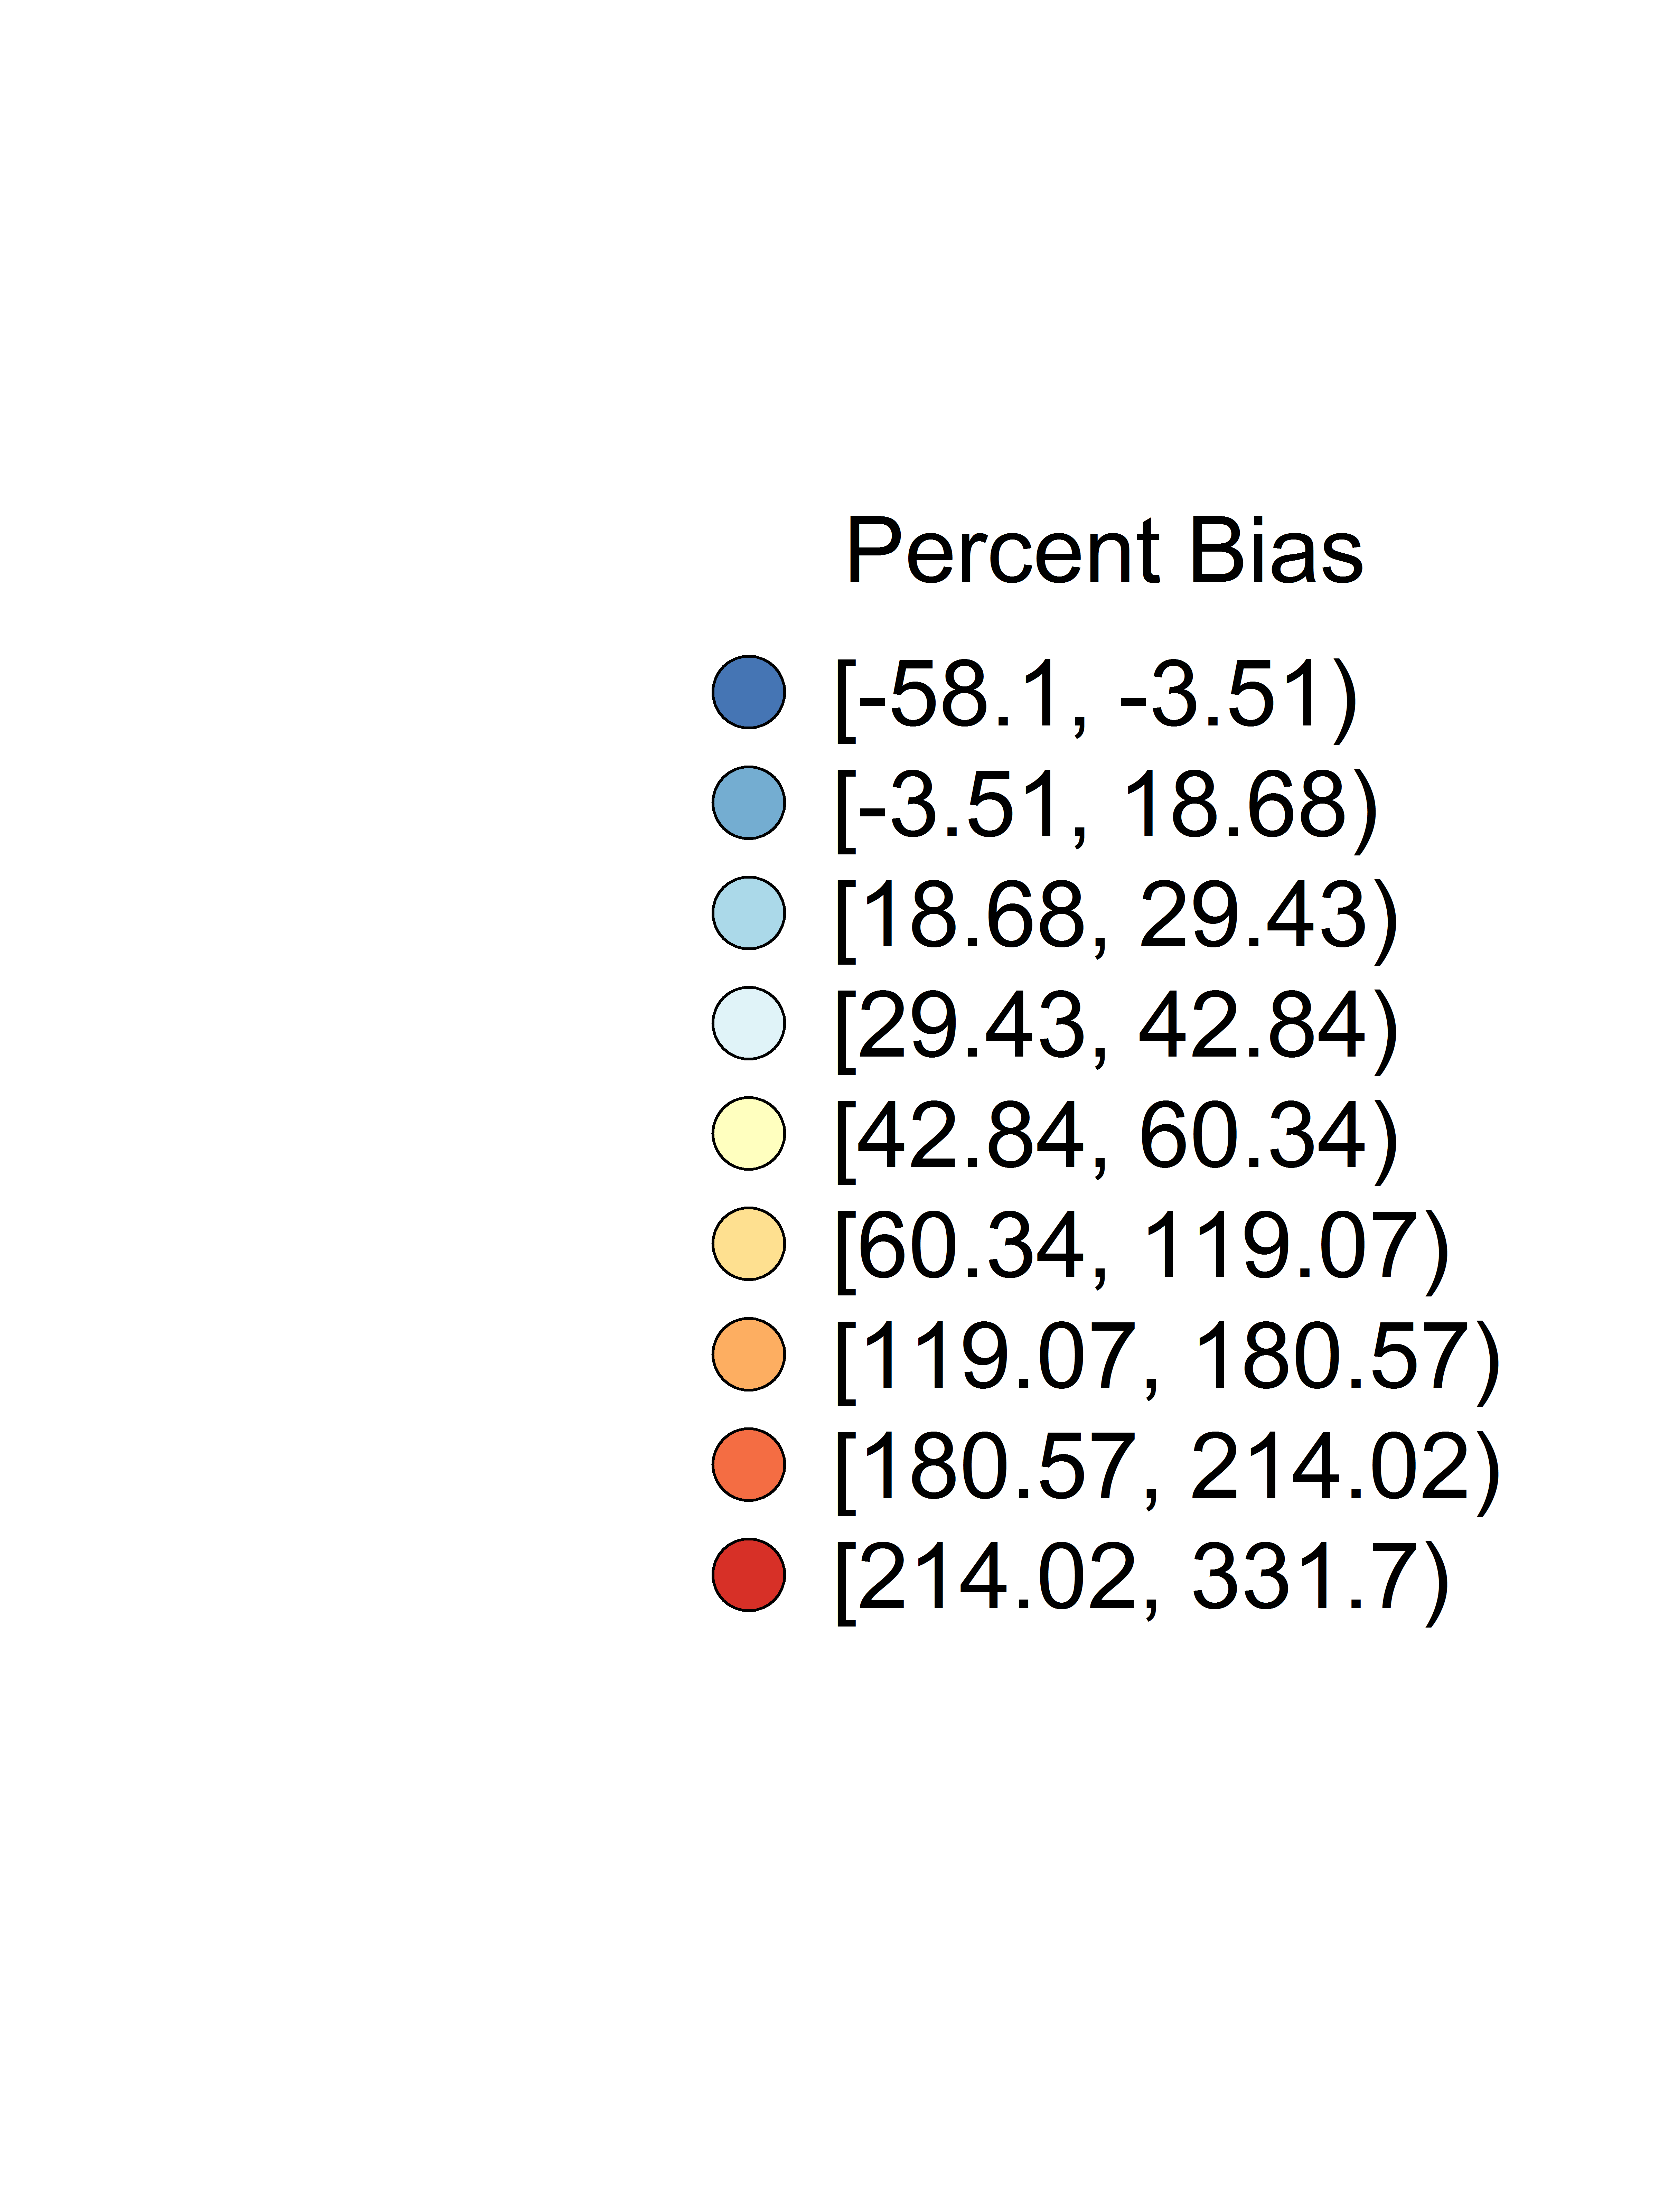
\includegraphics[scale=0.2]{./img/pbias_legend}
			% \caption{}
			% \label{fig:}
		% \end{subfigure}
		
%%%%%% for nash sutclif %%%%%%%
		% \begin{subfigure}[b]{0.3\textwidth}
			% 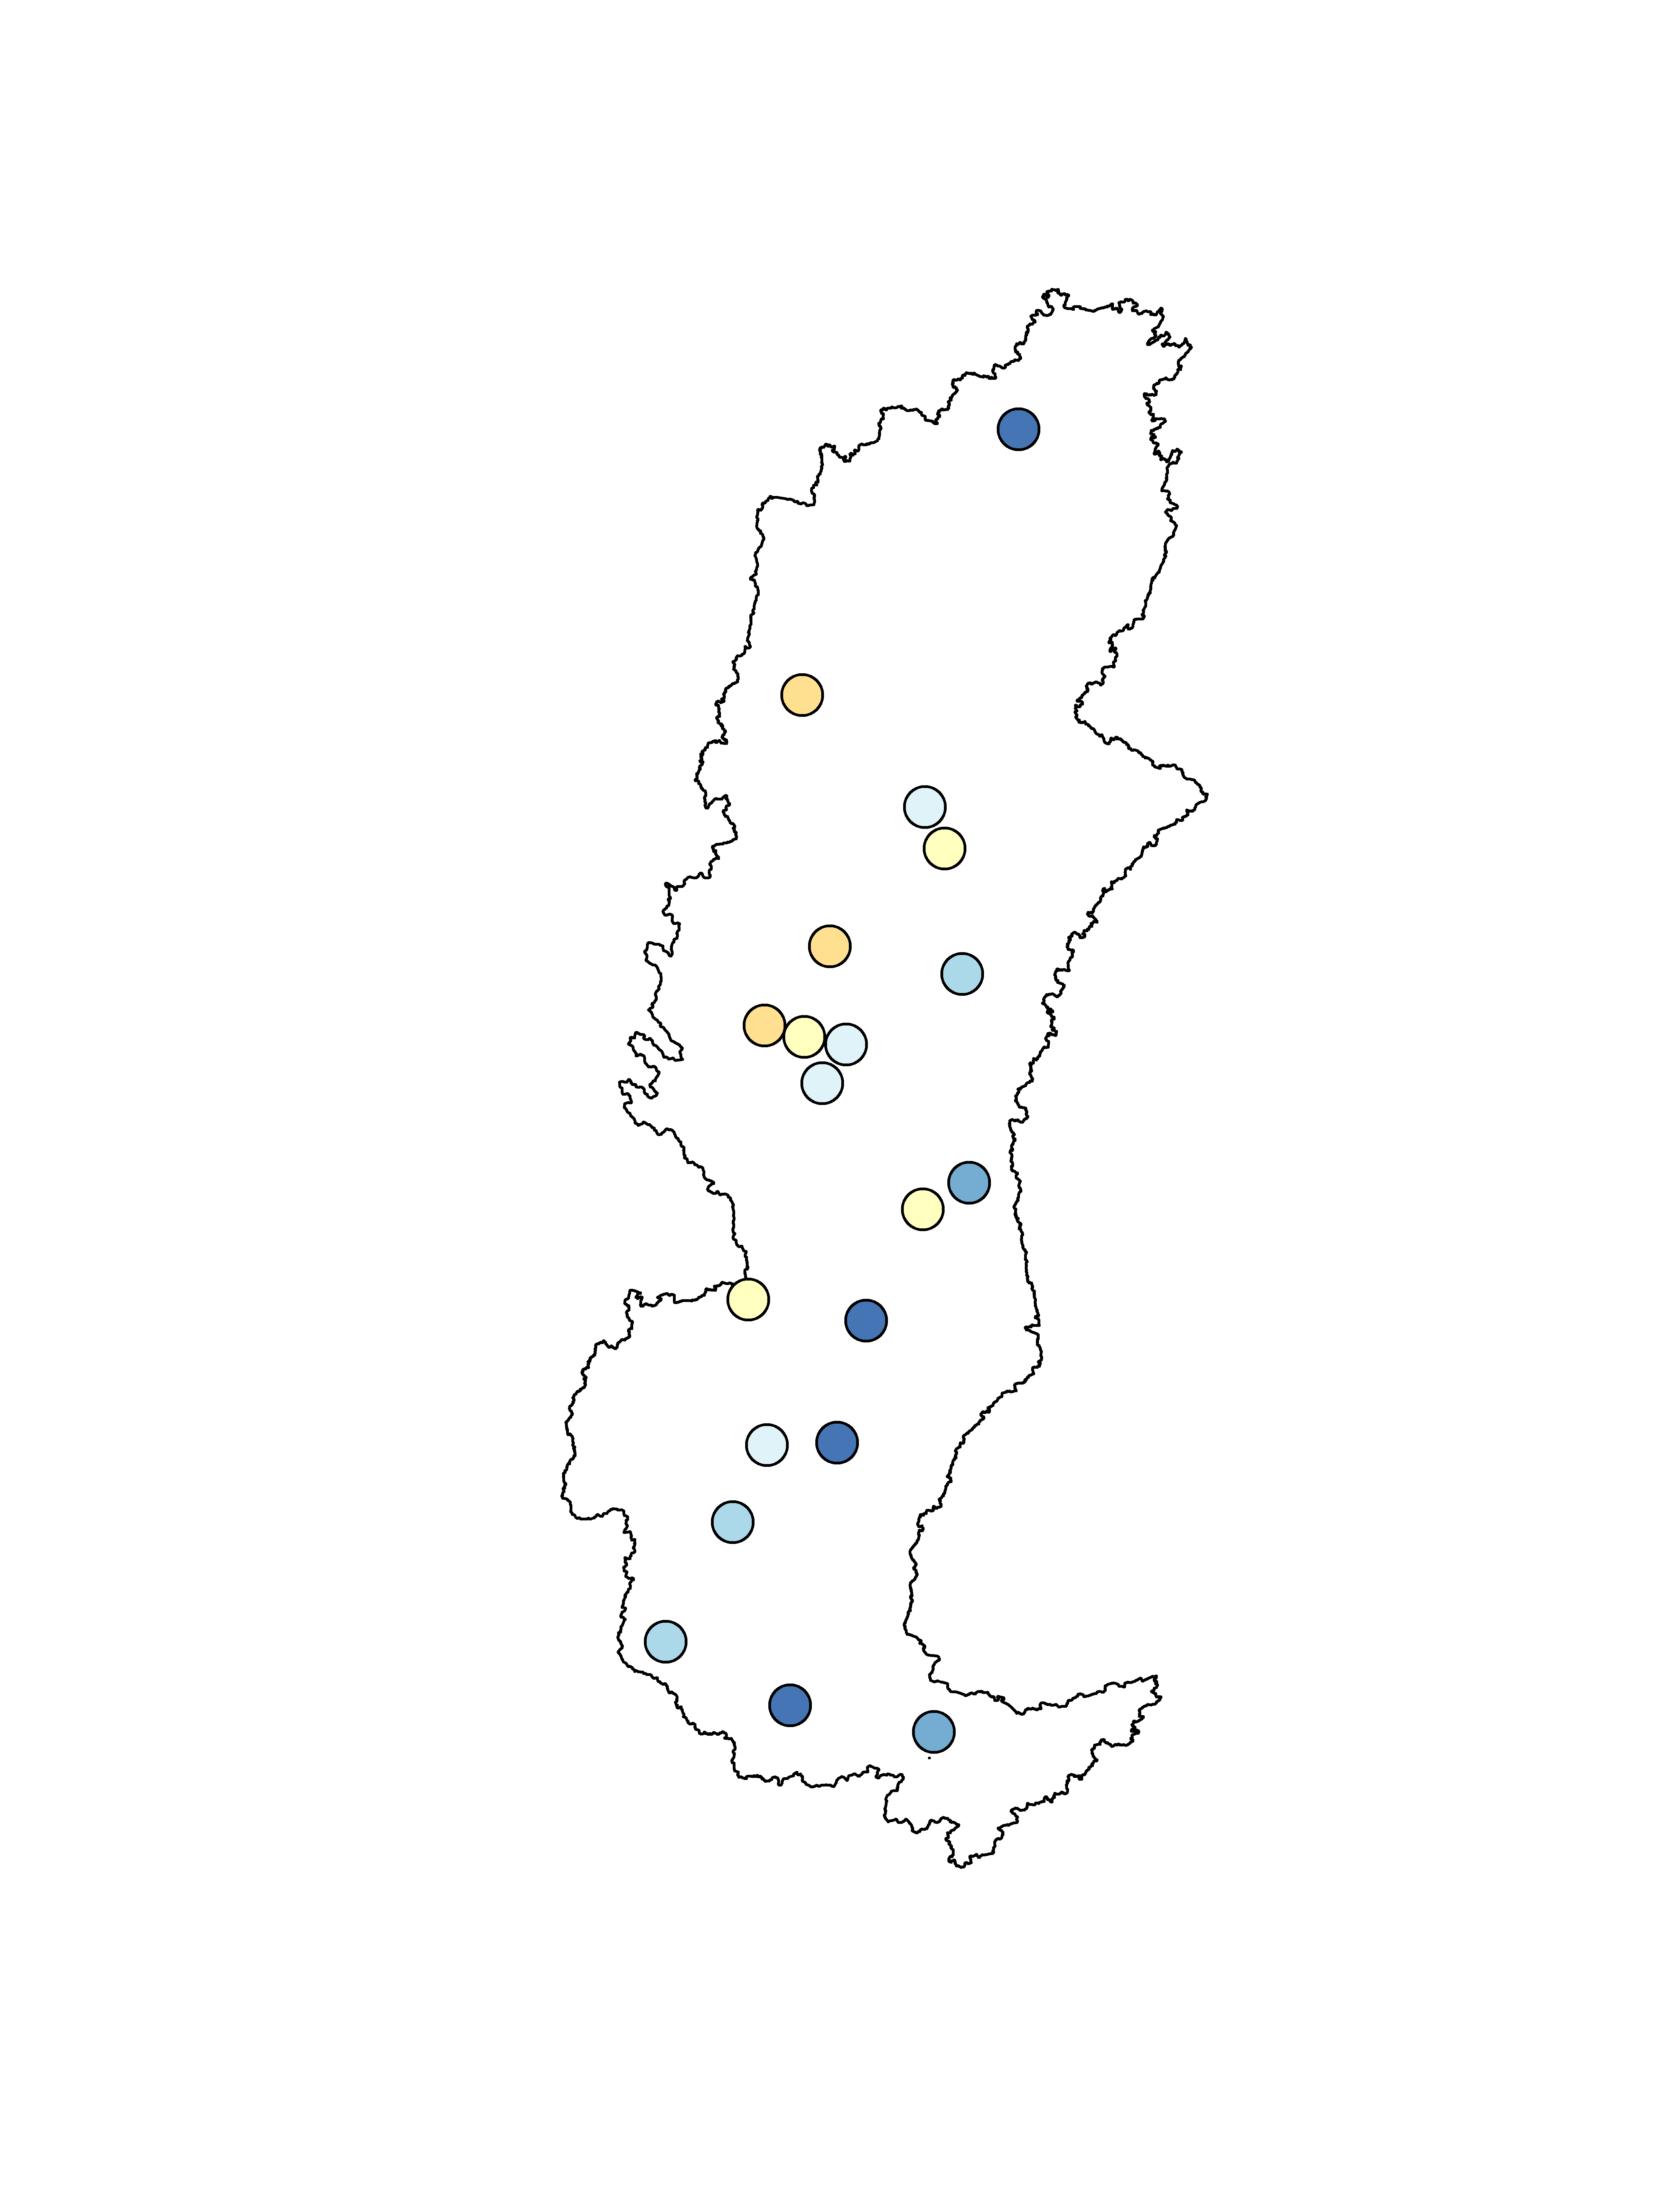
\includegraphics[scale=0.2]{./img/nashsut_harg}
			% \caption{}
			% \label{fig:}
		% \end{subfigure}
		
		% \begin{subfigure}[b]{0.3\textwidth}
			% 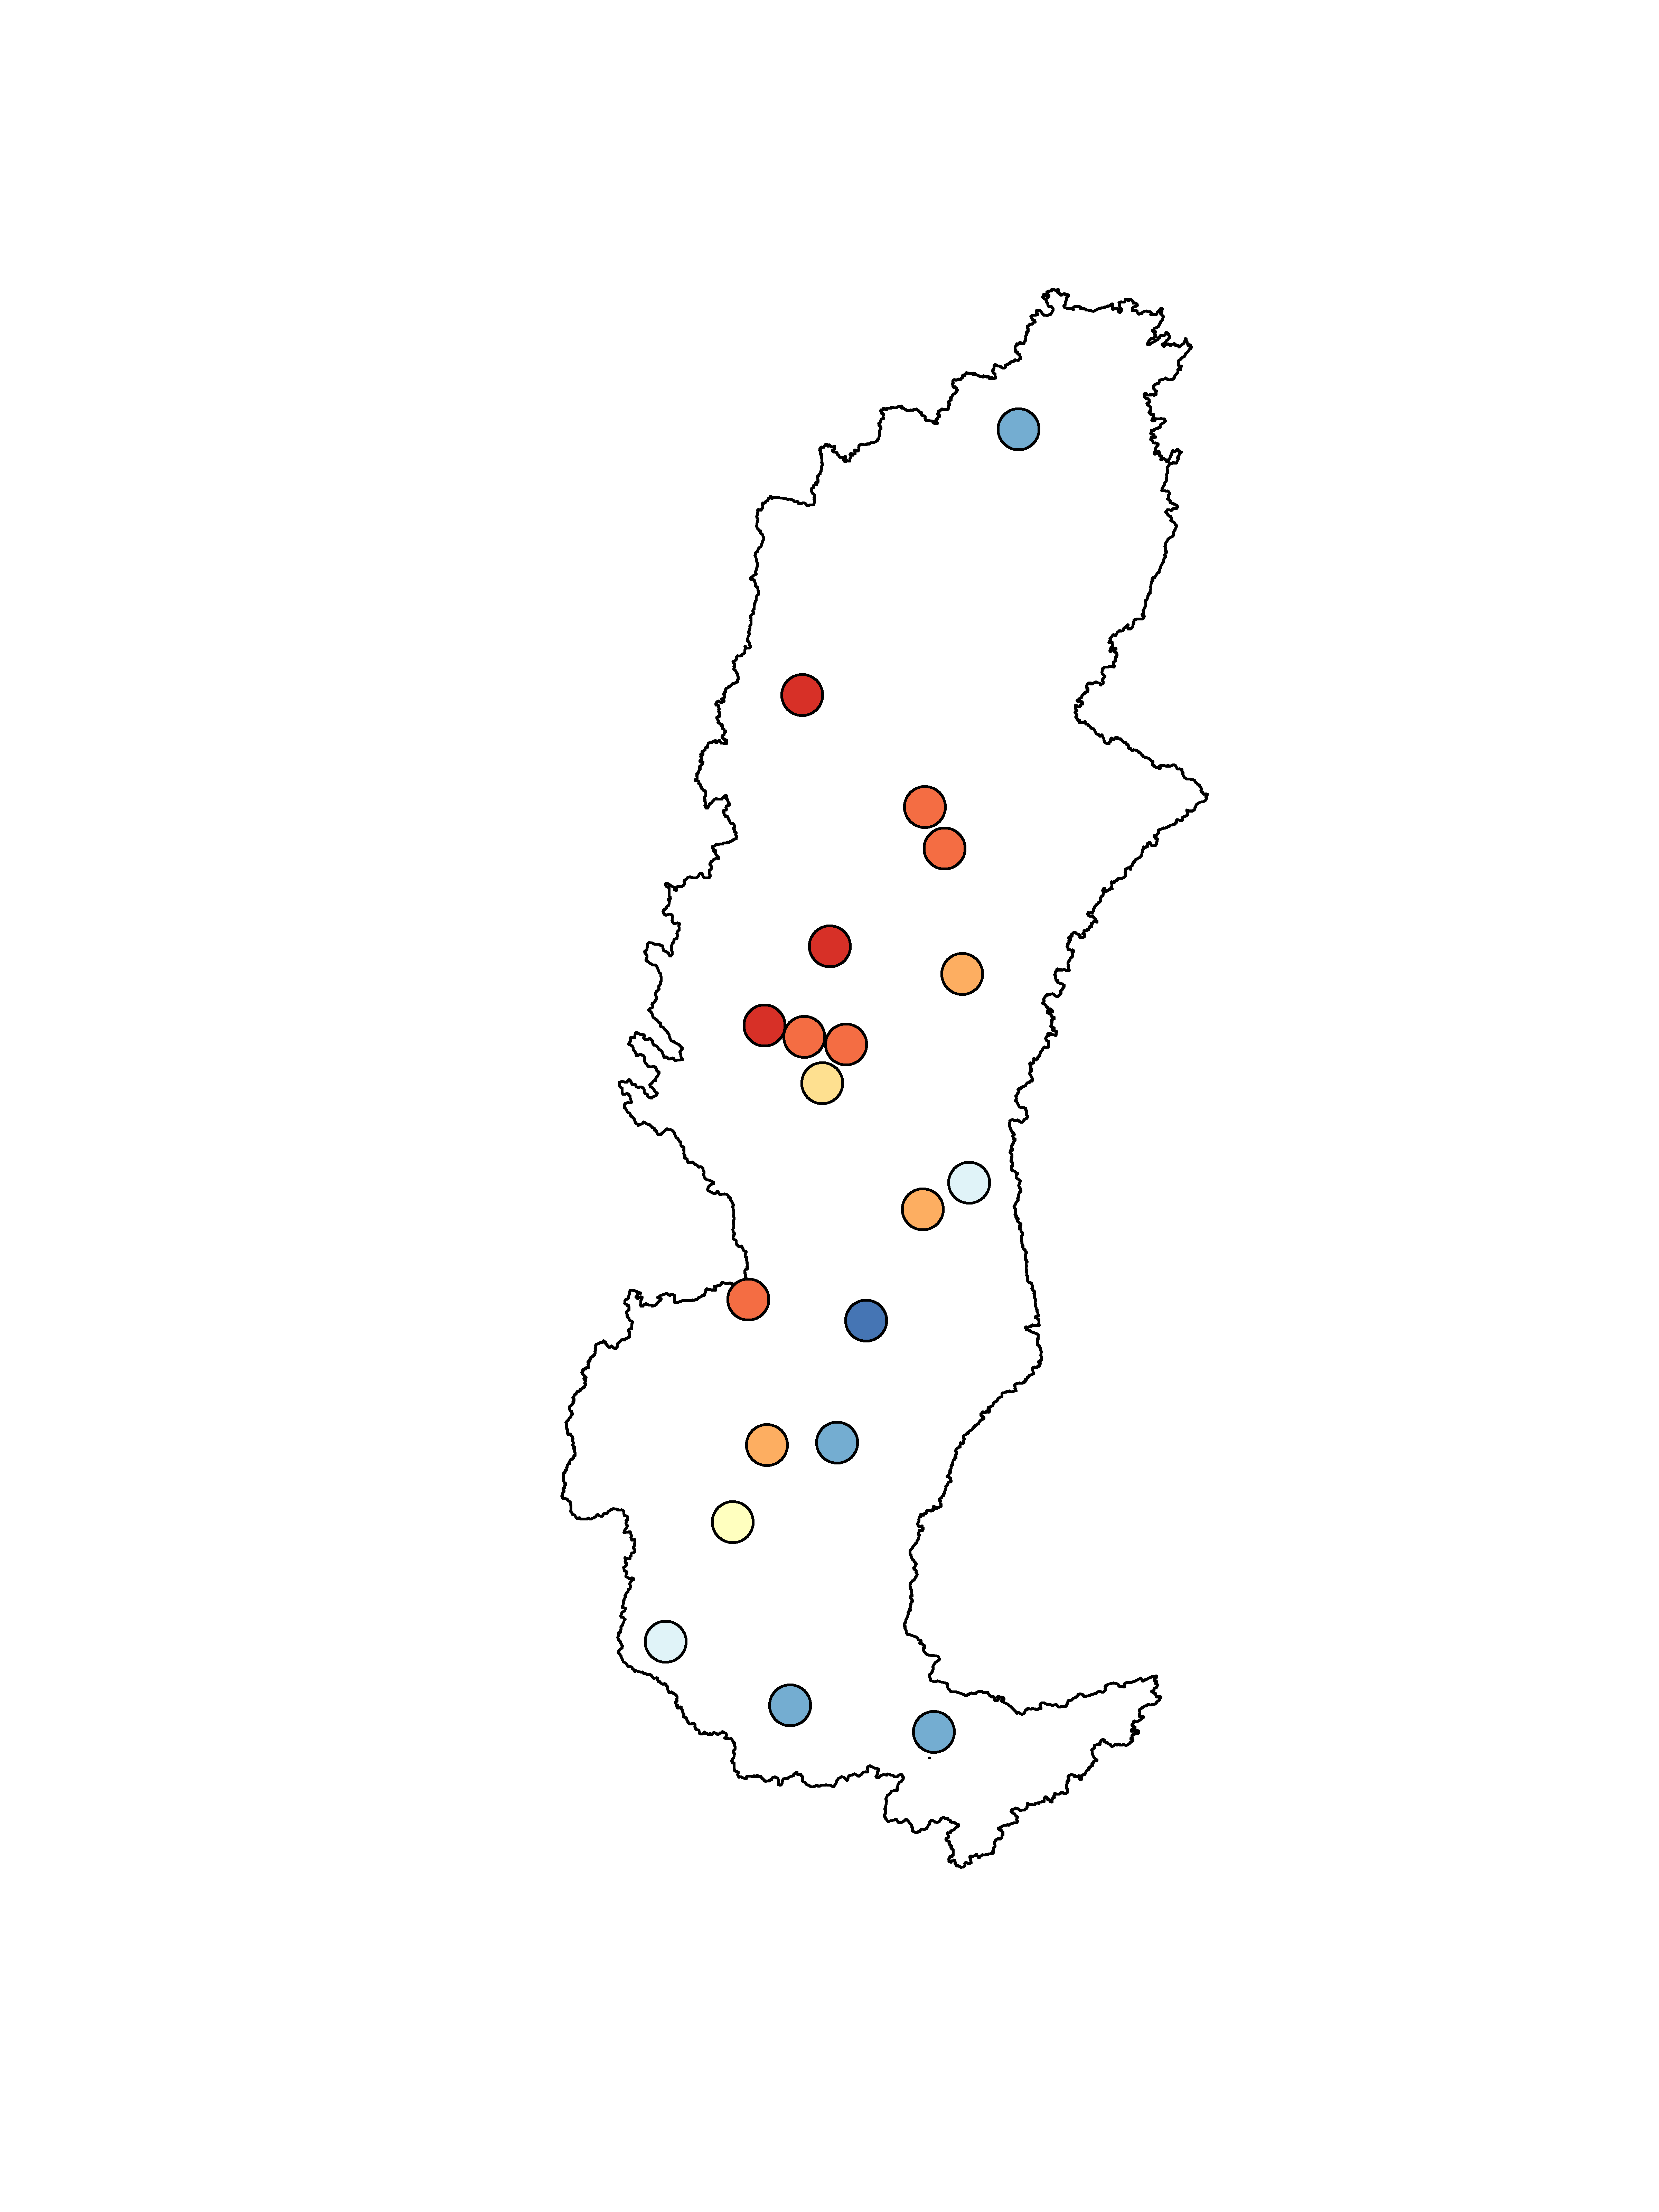
\includegraphics[scale=0.2]{./img/nashsut_penman}
			% \caption{}
			% \label{fig:}
		% \end{subfigure}
		
		
		% \begin{subfigure}[b]{0.3\textwidth}
			% 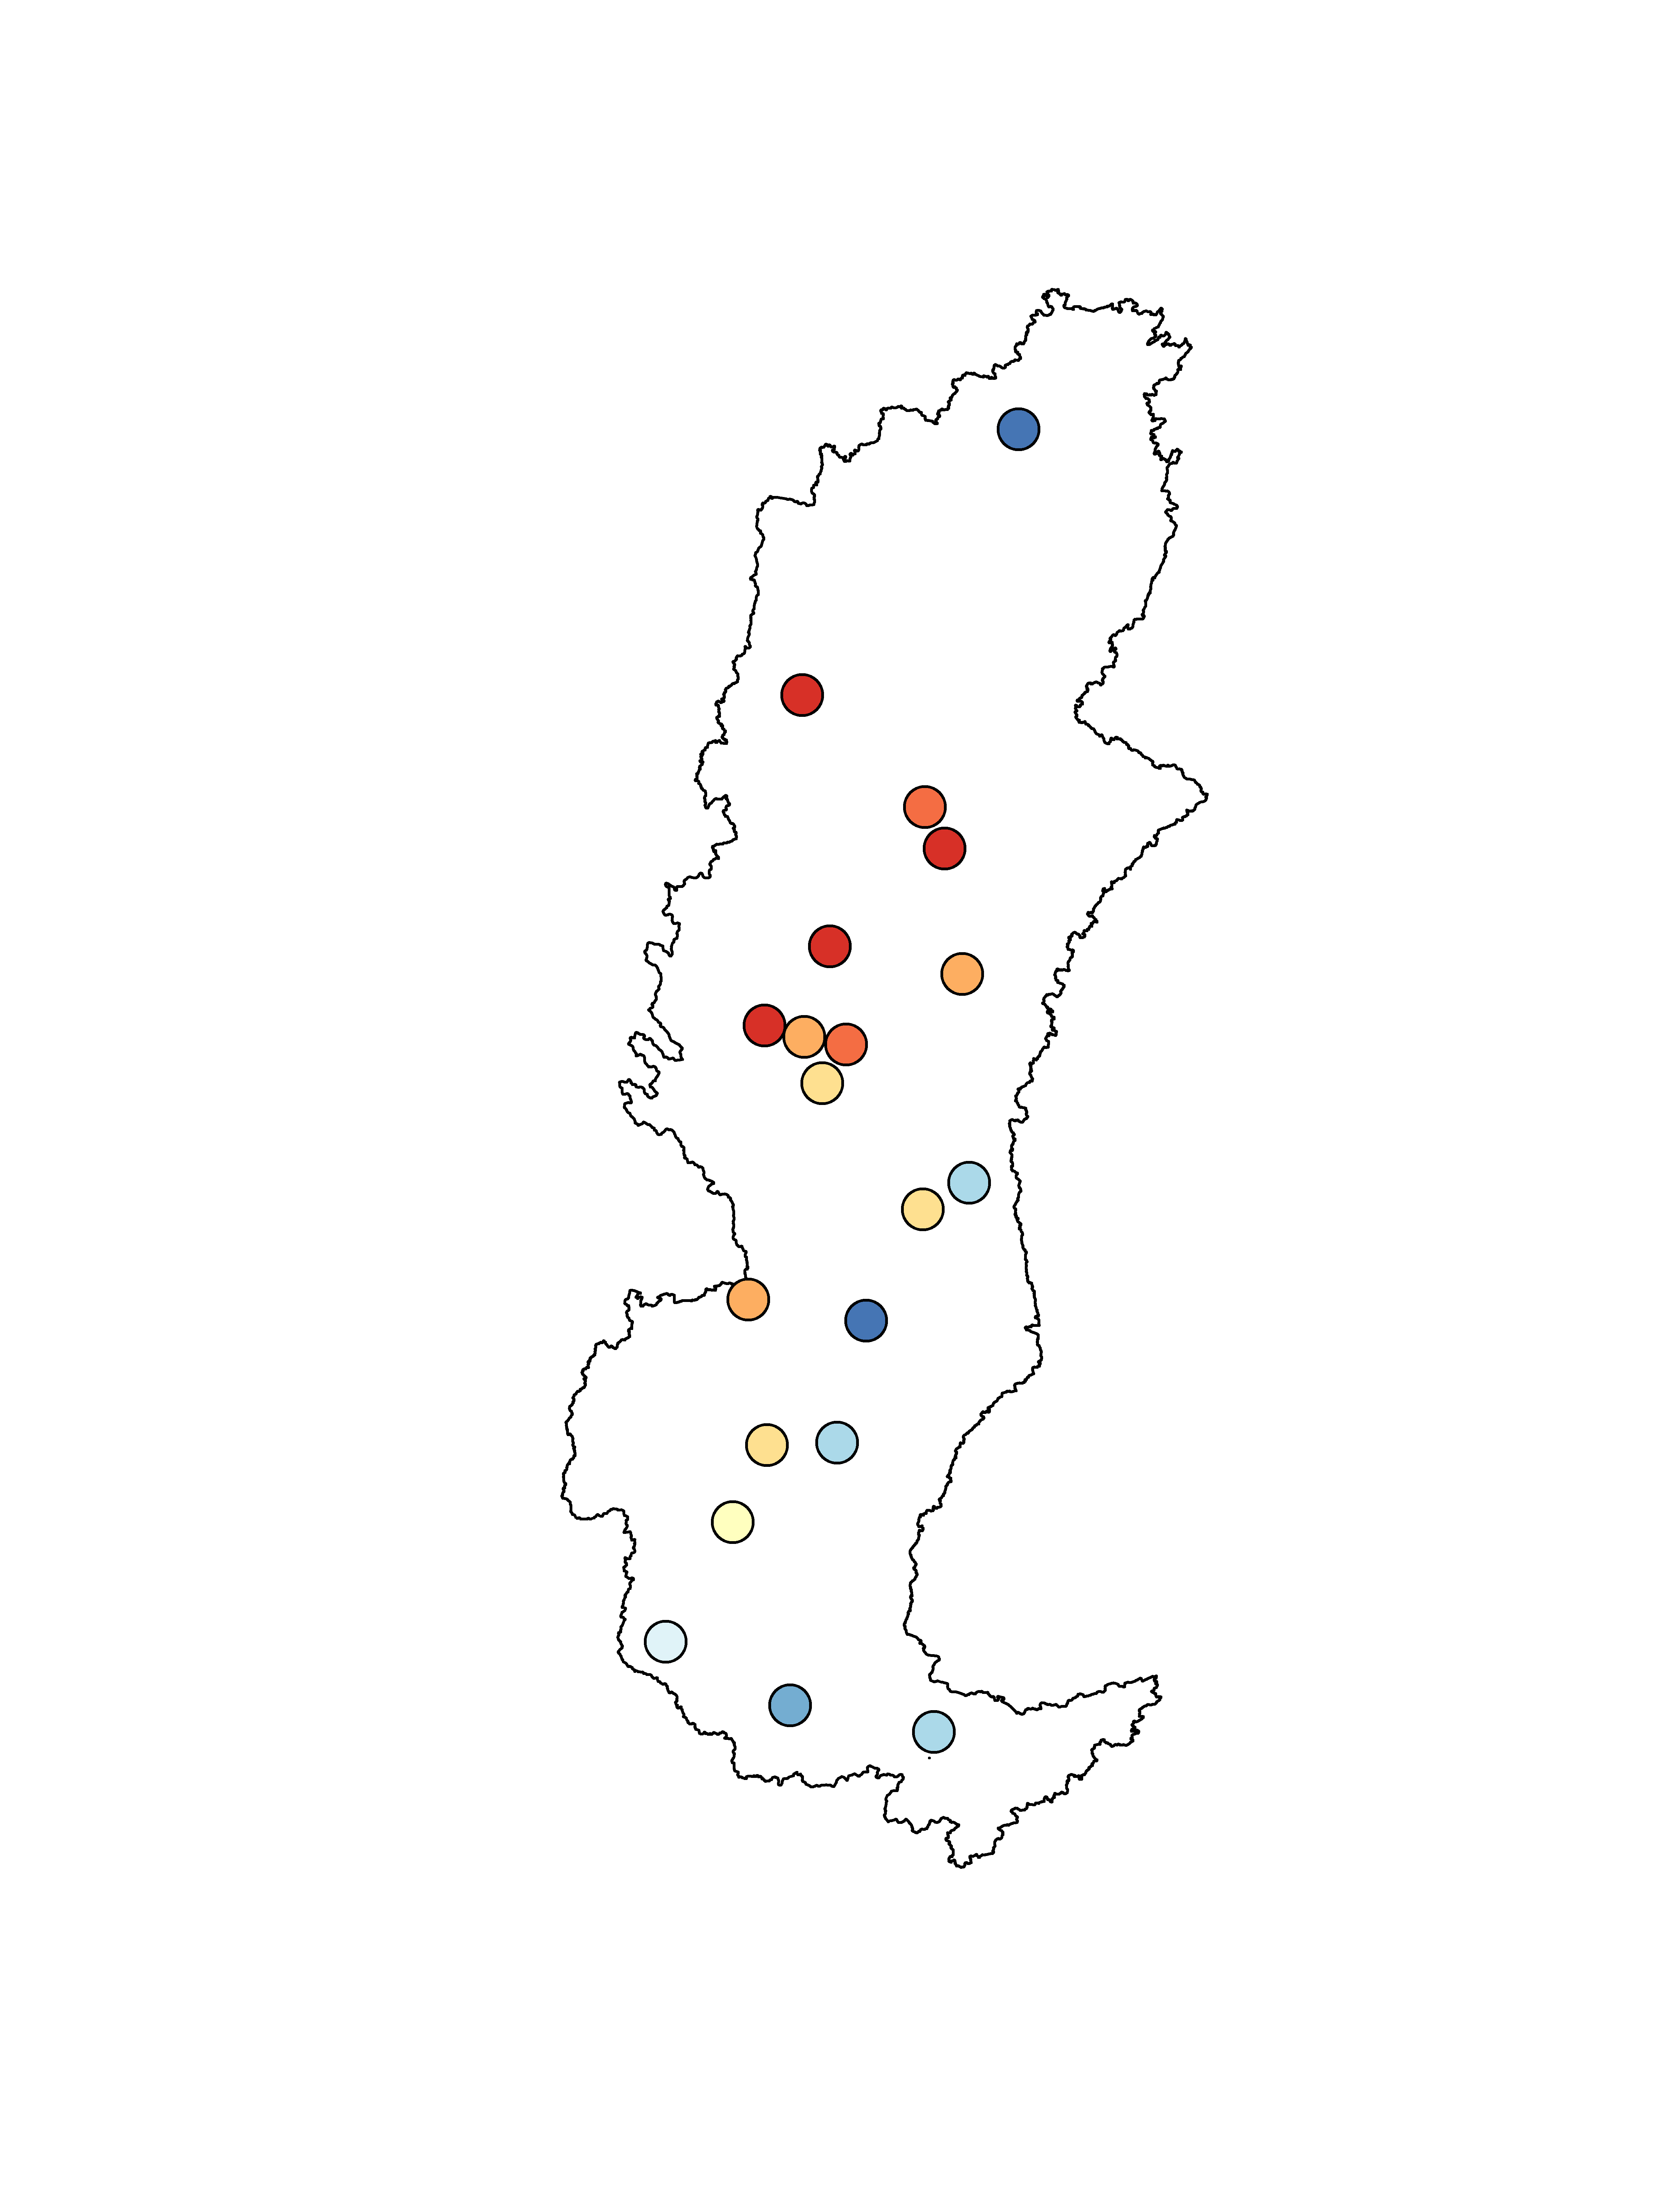
\includegraphics[scale=0.2]{./img/nashsut_priestley}
			% \caption{}
			% \label{fig:}
		% \end{subfigure}
%%		legend
		% \begin{subfigure}[b]{0.1\textwidth}
			% 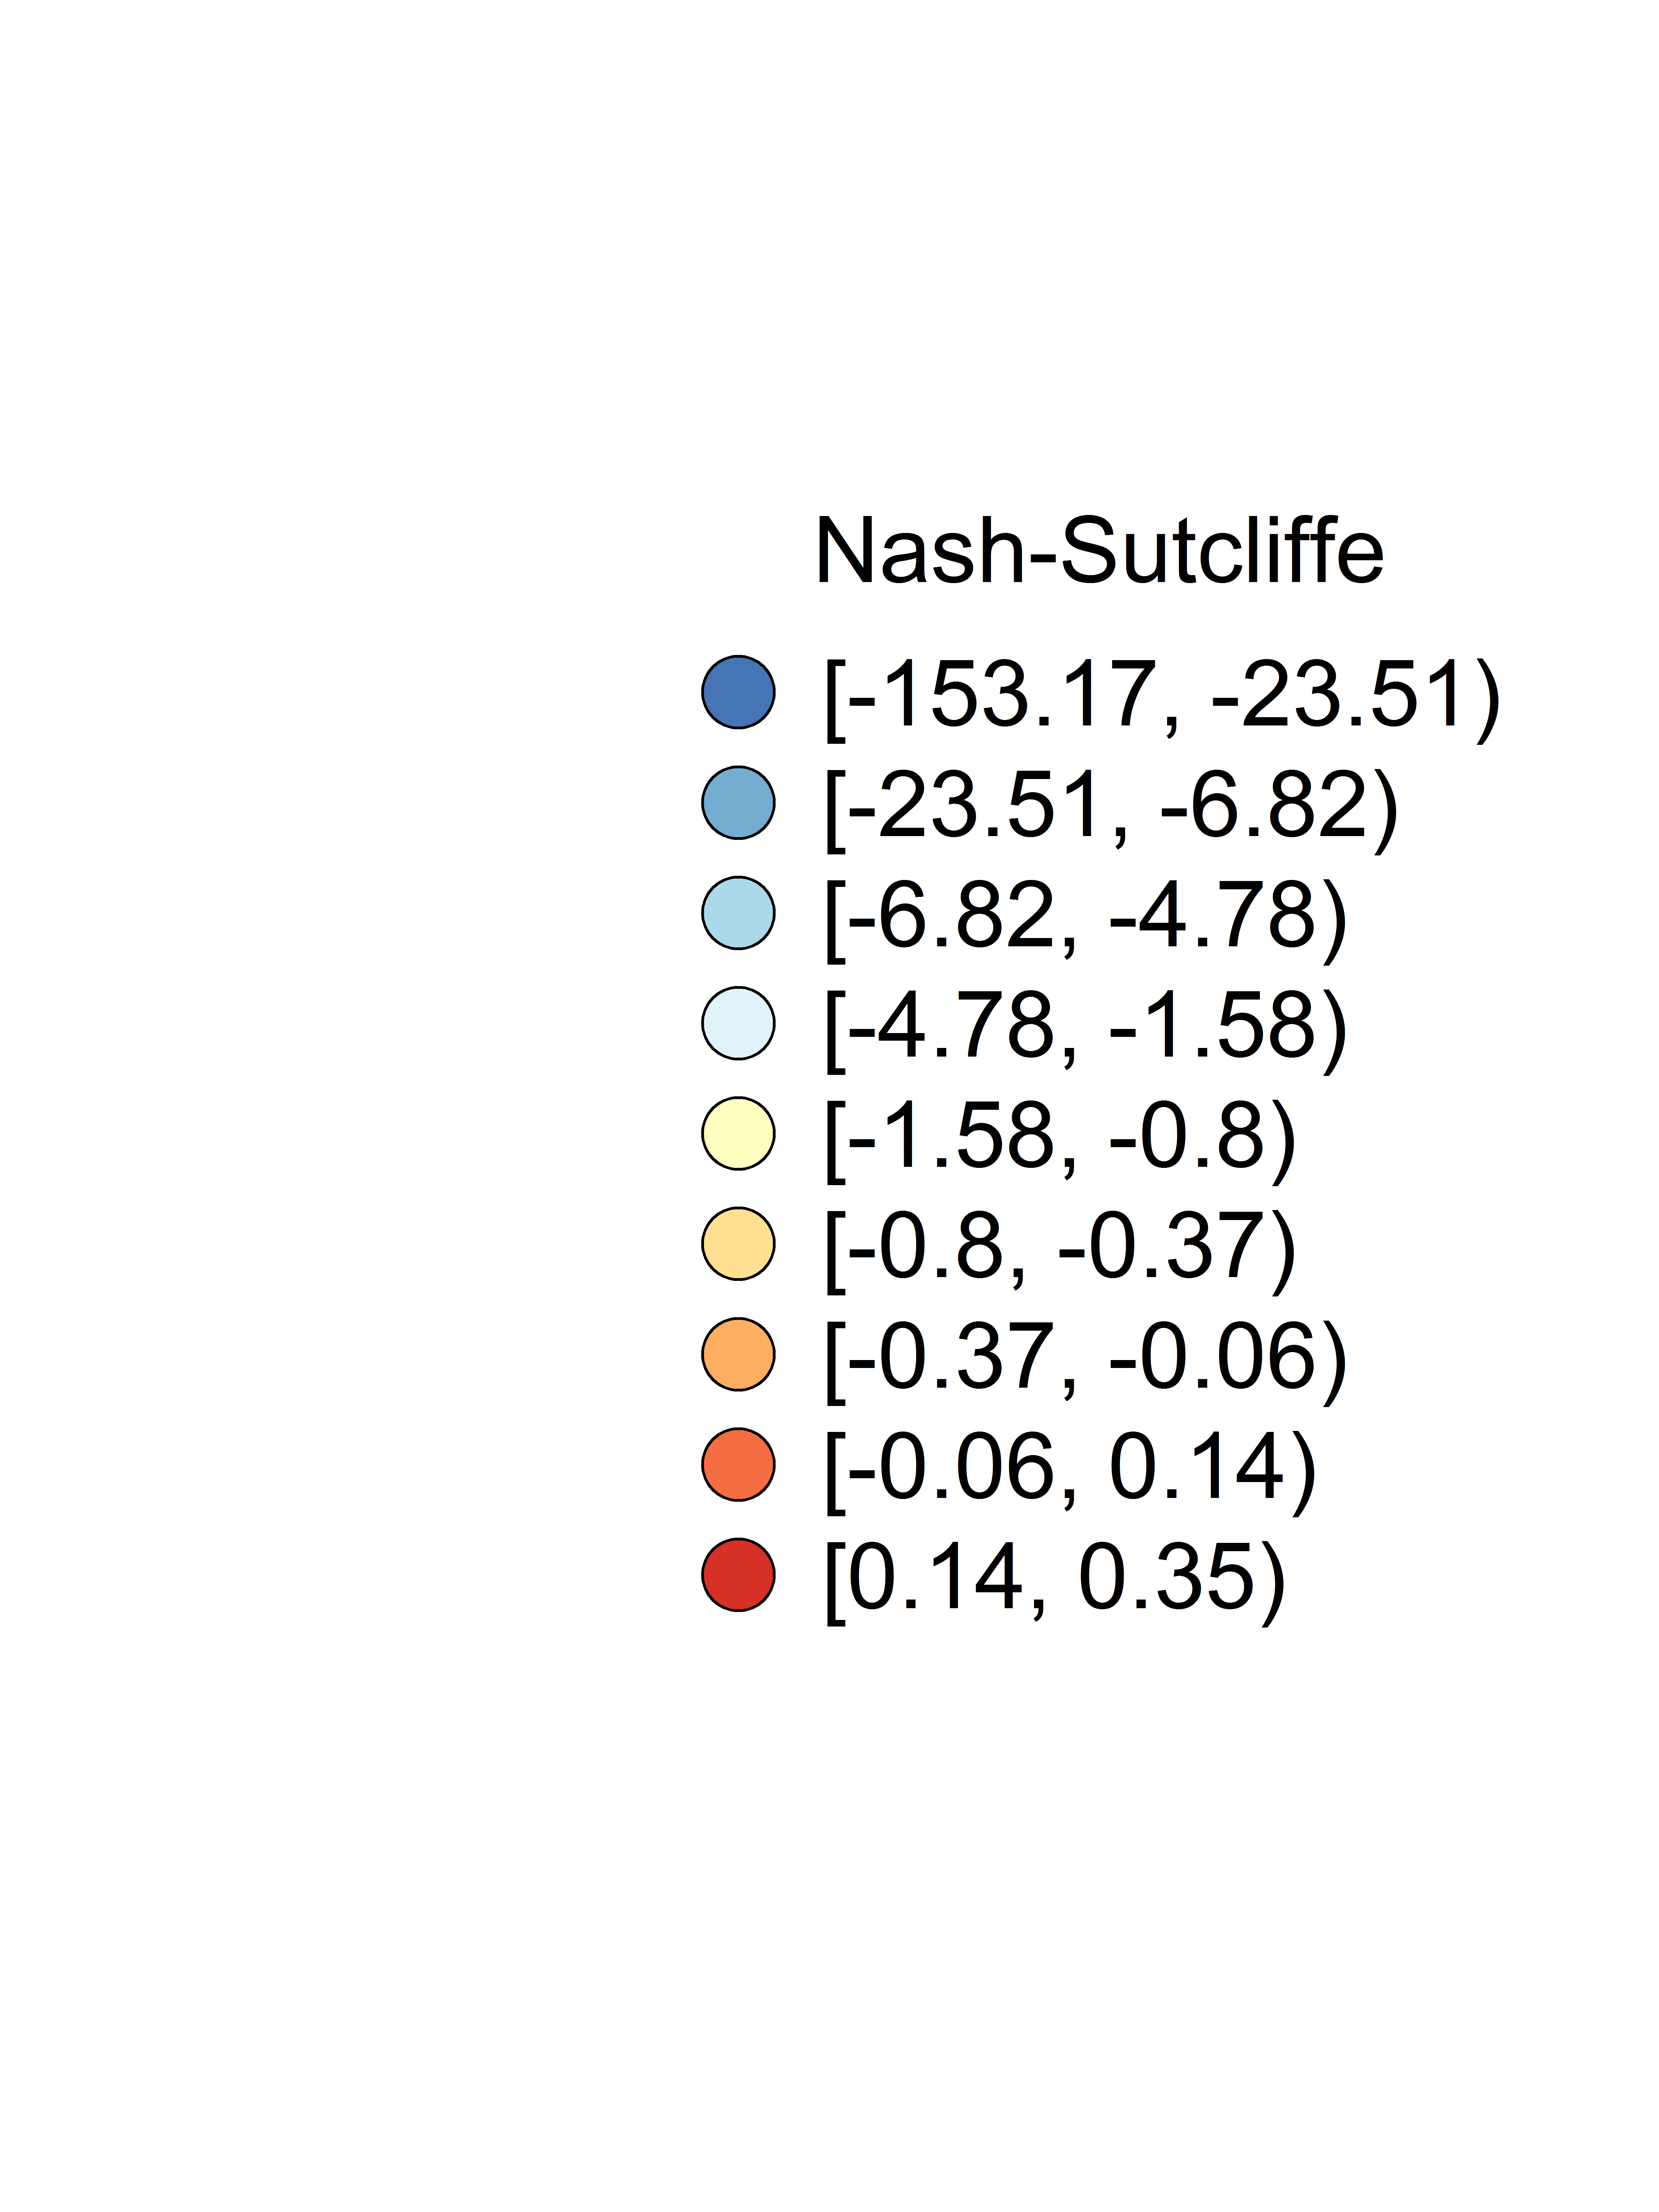
\includegraphics[scale=0.2]{./img/nashsut_legend}
			% \caption{}
			% \label{fig:}
		% \end{subfigure}
	% \end{figure}
% \end{landscape}






% \begin{figure}[h!]
         % \centering
         % \begin{subfigure}[b]{0.45\textwidth}
                 % \includegraphics{harv_Plots}
                 % \caption{{\small Harvel Field, N-rate plots on yield polygons}}
                 % \label{fig:woodstockPlots}
         % \end{subfigure}%
         % ~ %add desired spacing between images, e. g. ~, \quad, \qquad etc.
%           (or a blank line to force the subfigure onto a new line)
         % \begin{subfigure}[b]{0.45\textwidth}
                 % \includegraphics[width=\textwidth]{wood_Plots}
                 % \caption{{\small Woodstock Field, N-rate plots on yield polygons}}
                 % \label{fig:woodstockPlots_sand}
         % \end{subfigure}
         % ~ %add desired spacing between images, e. g. ~, \quad, \qquad etc.
%           (or a blank line to force the subfigure onto a new line)
%         \caption{Pictures of animals}\label{fig:animals}
 % \end{figure}r